%!TeX spellcheck = en-US

%\chapter{Web Genre Identification: A Survey}
\chapter{Relevant work}

\label{chap:relevant_work}

%----------------------------------------------------------------------------------------

% Define some commands to keep the formatting separated from the content
\newcommand{\keyword}[1]{\textbf{#1}}
\newcommand{\tabhead}[1]{\textbf{#1}}
\newcommand{\code}[1]{\texttt{#1}}
\newcommand{\file}[1]{\texttt{\bfseries#1}}
\newcommand{\option}[1]{\texttt{\itshape#1}}

%----------------------------------------------------------------------------------------

\section{Introduction}\label{chap:relevant_work:sec:intro}

\section{The Notion of Genre}
\label{chap:relevant_work:sec:definitions}

In general, genre is related to form and communicative purpose of texts rather than their theme. It is closely related to style and \textit{Genus}\footnote{Genus in Greek means \textit{type} or \textit{class}} \parencite{sugiyanto2014term}. Approaches to define text genre start mainly from two directions: linguistics and computational analysis of language (e.g. computational linguistics, natural language processing, text mining). 

In studies of linguistics there is a great debate in defining the notion of genre as an abstract categorization scheme of texts and the relations between them. Despite the methodological differences the linguistic community concluded that the idiosyncrasy of the \textit{genre taxonomy} is mutable and diverse \parencite{coutinho2009describe}. This kind of idiosyncrasy is yielded to the genre taxonomy due to the spontaneous genesis of the genre classes. The genesis of a genre class is a socio-centric interaction which is emerging from the need to describe the texts in order to accelerate the social communication procedure. Thus, genre classes are spontaneously emerging while the communication procedure is taking place.

Humans can efficiently recognize the genre-types by processing the texts intuitively. However, there is a lack of consensus for defining genres, particularly when specific names (labels) should be assigned to the genres. There there was an effort of several user studies for eliciting the mechanics in the process of genre identification and tagging. The results on user agreement were very discouraging. Also, when humans attempt to describe specifically the terms or/and the attributes which they use to identify different genres, there is a great confusion and disagreement. A convincing explanation for this is the plethora of textual, stylistic and conceptual description terms which humans use and depend on their background (e.g., teachers, scientists or engineers use different vocabularies to describe texts belonging to a common genre \parencite{roussinov2001genre, crowston2011problems}. 

Researchers from cognitive science found that humans are recognizing the genre type of a document (or web-page) using cognitive processes related mostly to the form of the text. Particularly they used configured apparatus for tracking the eyes movement while subjects attempt to recognize genre of documents. One can resemble the process like navigation where the eyes are constantly moving while they are focusing for small fragments of time in landmarks of interest. The pausing of the eyes on the text "landmarks" is called \textit{fixation} while the "jumping" movements of the eyes is called \textit{saccadic}. The whole process aimed to locate information of interest such as specific text forms, names, verbs, or phrases that are related to the abstract concept in order to decide whether the text matches their interest and is worth of further reading. They systematically found that the process of finding the genre-type of the text is the same as to find out whether a text id worth of further reading. Thus, the knowledge of a genre taxonomy definitely accelerates the communication procedure and helps readers of the text to find the information of interest faster \parencite{clark2014you}.

The discipline of the \textit{English for Academic Purposes} (EAP) has vividly discussed the divergence in the genre taxonomies between the different academic disciplines and reasoned the utility of the genre taxonomy for enabling the teachers and the students to improve their rhetorical and written language skills with the purpose of improving the teaching procedure. What is important to note for this study is the conclusion that any given certain genre conveys information about the communication purpose of the document, i.e. as text identity carrier, but it can also contain the same style and other language properties when the purpose is similar. For example, the article of newspaper and an article from a magazine can be claimed to belong to different genres although they are mainly governed by the same linguistic properties. Therefore, for the witter of a text is is very important to be aware (thus to be taught) of the different genres and the taxonomy of genres in order the text (s)he produces to be recognizable by the reader \parencite{hardy2016genre,melissourgou2017genre,al2017genre}. However, genre itself requires different level of human reading abilities to be recognized and even with these skills different humans may disagree \parencite{mccarthy2009psychological}.

The utility of text genre identification has been realized by the journalism professionals. There are well-defined structures and guidelines given by newspaper editors about how to present, e.g. news articles. The structure consists of abstract elements and they follow specific paradigms, like the \textit{inverted pyramid} (i.e., contents are structured from the most important to the least important information), \textit{Martini Glass} (i.e., it first presents a summary of the story, then an inverted pyramid and finally a chronological elaboratio), \textit{Kabob} (i.e., it starts with an anecdote, continues with the main story and closes with a general discussion) and \textit{Narrative} (i.e., it presents a chronological sequence of events) \parencite{dai2018fine}.

From a computational analysis point of view, genre (and genre taxonomy) is important as a classification factor to distinguish between documents. Genre labels are defined according to their association with practical applications rather than based on a rigid theoretical background \parencite{kanaris2009learning,santini2007automatic}. Genre identification is a style-based text categorization task. Another similar task is authorship attribution where the focus is on identifying the \textit{personal style} of the author \parencite{stamatatos2009survey,koppel2011authorship,koppel2014determining}. On the other hand, genre is mainly regarded as a \textit{group style}. Foe example scientists use a common form of language to write research papers, journalists describe news events and their opinion using similar patterns, bloggers express their beliefs and interests based on similar structures, etc.

As concerns web genres (and their respective taxonomy), the utilities and opportunities that can provide as well as the difficulties they impose have been eloquently analyzed. It has been pointed out that the genre taxonomy summarizes the type and style of texts in a single term as a communicative act \parencite{de2009genre}. In the domain of WGI, usually a web genre palette is defined usually obtained from a top-down approach, where a group of domain-experts design the taxonomy based on specific objectives of the task \parencite{crowston2011problems}. Moreover, the genre palette may flat or hierarchically-structured \parencite{wu2010fine}. The former assumes that genre labels are independent while the latter defines a hierarchy of genres and sub-genres. Another important issue is whether a web-page should belong to exactly one genre label or page segmentation should be applied first and then each segment should be assigned to a genre label  \parencite{madjarov2015web,jebari2015combination}. 

As described so far, there is agreement for the criteria which are defining the genres (and web genres) in a given domain. These are, the style, form, and the communicative purpose of documents. In theory, topic is considered orthogonal to genre. However, thematic information can also be useful in automated genre identification. For example, the genre of academic home web-pages is distinguished by a specific vocabulary. The genre of research papers also use specific science-related terms. Certainly, some of these terms may be too specific (e.g. about biology, mathematics, or computer science). However, content-specific information can be used to differentiate scientific documents from non-scientific documents \parencite{coutinho2009describe,crowston2011problems,kanaris2009learning,jebari2015combination,gollapalli2011identifying}. 

Considering the above discussion, it is clear that the notion of web genre depends on the use of this information. In this thesis, our approach is influenced by the use of web genres as a classification factor in order to enhance the potential of information retrieval systems. In particular, we use the following definition:

\begin{definition} A web genre is a class of web documents. Every web-page is always derived under a unique class distribution and the class distributions are not overlapped.
\end{definition}

\section{Representation of Genre-related Information}

\subsection{Textual Features}

The \textit{Superficial Document Characteristics (SDC)} can be considered as features and document representations together where they are the counts of the Words lenghs (in characters) frequency, the Sentencies length (in words) frequency, the Paragraphs length etc. In addition the Max, Min, and Ratios of these SDC were also count such as the \textit{Average to Max size of Words Ratio, the Max Word Length Frequency} etc. In general several facets, i.e. \textit{terms types}, have been tested for WGI cornering the Hypertext \parencite{feldman2009classifying,santini2005linguistic}.

To begin with, it shown that the \textit{Writing Style Features} and \textit{Key Event Placement (KEP) Features} are improving significantly the performance of the SVM classifier \parencite{dai2018fine}.  The writing style features are extracted as a combination of  other complex features, i.e. the combination of \textit{grammar production rules (GPR} and features from a semantic category of a \textit{Linguistic Inquiry and Word count (LIWC)} dictionary. GPR are the combination of POS and word lexical rules. LIWC is a sophisticated dictionary of occurrences of word from a word category. The KEP is a set of text formatting features, or "landmarks", such as \textit{specific characters, time, location} at specific areas of the text. In practice it is the \textit{words overlapping count} between the \textit{first paragraph} and \textit{the title} of a document. The combination of these structured based features has improved the macro-F1 performance.

As registers are also considered as genres then there is also a set of heuristics have been used for a classification for this taxonomy. Particularly in \parencite{onan2018ensemble} Language Function Analysis (LFA) has been introduced for a classification task on a taxonomy of \textit{Expressive, Appellative,} and \textit{Informative} classes. The LFA is combining features that successfully used for Authorship Attribution (AA), Linguistic Features (LF), Character n-grams (CNG), Part of Speech n-grams (POSNG), and the frequency of the most discriminative words (MDW). 

\begin{itemize}
\item Features used in authorship attribution (AA) usually are words, POS n-grams, character n-grams, capitalized words, lowercase words frequency, punctuation and quotation marks frequencies. 
\item Linguistic features (LF) usually are time and money entities, POS, personal pronouns, possessive pronouns, adjectives and nouns frequencies. 
\item Character n-grams (CNG) usually means their frequency of the n-grams, over a specific frequency threshold, say at least 4 times occurrence. 
\item Part of speech n-grams (POSNG) same as CNG but for POS.
\item The frequency of the most discriminative words (MDW) this is usually task dependent.
\end{itemize}

The \textit{Textual content} is the most analyzed part of the hypertext which has been used for WGI \parencite{mason2009distance,Sharroff2010}. There are several features than can be extracted used alone or combined to getting the maximum information one can get from the web-paged and feed it for training a prediction ML algorithm. Character n-grams, Word n-grams, Part-of-Speach n-grams and some \textit{special discriminative words} have been commonly used and usually combined with some heuristically extracted features \parencite{kanaris2009learning,kumari2014web,levering2008using,Lim2005,mason2009n,onan2018ensemble,petrenz2011stable,sharoff2010web,Nooralahzadeh2014}.

\parencite{waltinger2010feature} The features suggested (but not constrained) for this algorithm and for the WGI task are the following:

\begin{enumerate}
\item Word n-grams, Character n-grams, Word uni-grams and POS n-grams
\item Superficial and Structural such as the sentence length and the divisions number, and the paragraph length, concerning of the HTML text formatting.
\item HTML tag frequency in their logical structure, e.g. the number of <p></p> tags in total by ignoring the special cases of attributes or style sheets than might contain individually.
\item HTML Attribute Frequency same as in tags case.
\item First-Last tag frequency the x number of  the first occurring html tags and the y number of the last occurring tags.
\item Name entities frequency based on an entity recognition heuristic engine.
\end{enumerate}

In order to take into account all the above features contribution to the WGI task, a \textit{weighted sum all the} $IM^{k}_{mn}$ scores is calculated by the equation \ref{eq:ranking_distance_weighted_sumsum}

\begin{equation}\label{eq:ranking_distance_weighted_sumsum}
	C_{g} = \sum_{k=1}^{F} \delta_{k} \cdot IM_{mn}^{k}
\end{equation}
Where $C_{g}$ is the similarity score for the a genre of the taxonomy, and $\delta_{k}$ is the weight of the $k$ feature set from all $F$ features, where is under the constraint co $\sum_{k=1}^{F} \delta_{k} = 1$.


\subsection{Readability Assessment Features}

Readability Assessment Features (RAF) have also been tested for the WGI/AGI task. Moreover, a primitive attempt also presented related to these features where they have been evaluated (and compared to other features) in their effectiveness on different taxonomies. Particularly they compared on the \textit{Domain-taxonomy} and the \textit{Genre-taxonomy} \parencite{falkenjack2016exploratory}.

Although, there is a ambiguity in the research literature related to the Domain/Genre definition, usually the genre considers to be (as explained in section \ref{chap:relevant_work:sec:definitions}) more abstract and related to \textit{the texts organization, rhetorical structure, length, syntax, morphology} and \textit{vocabulary richness}. Domain is more related to the \textit{General topic of a group of text}. Consequently, \textit{Sports} as category is considered to be a Domain while \textit{Academic papers} are considered Genres.

It has been shown that genre-taxonomy ML classification is benefit by the use of RAF while the domain-taxonomy does not. 

The RAF are very old in because they are studied since 1920 where their main purpose is to help in the evaluation of a text in respect the ease in reading and comperhation by the abilities of the reader. Although, the function includes two (2) variables the research is mainly focusing on the aspect of the evaluation of the text side only. 

The most basic metrics are LIX metric (see eq \ref{chap:relevant_work:eq:LIX}) , OVIX (Word Variation Index) and NR (Nominal ratio) metric. However, since the evolution of ML there are several other text information have been evaluated and also used in combination with the basic metrics \parencite{falkenjack2013features}.

\begin{equation} \label{chap:relevant_work:eq:LIX}
	LIX = \frac{A}{B} + \frac{C \cdot 100}{A}
\end{equation}
\nointend where $A$ is the number of words, $B$ is the number of special characters (i.e., colon, period, capital fist letter), and $C$ is the number of long words (more than 6 letters for the English language). 

RAF other than the basics are including some \textit{Superficial features, Lexical features, Morpho-syntactic features} and \textit{Syntactic features}. Specifically the selected features from every lingustic categories are:

\begin{enumerate}
\item Superficial: Average Word Lengh (in Characters), Averga Word Length Syllables per word, Average Sentence Length.
\item Lexical: Vocabulary Lemmas for Communication, Everyday use, High frequent, Unique.
\item Morpho-syntactic: Unigram-POS, ratio-to-content of nouns, verbs etc.
\item Syntactic: Average Dependency Distance, ratio of Dependencies, Sentence Depth (in dependency terms), Unigram Dependency Type (based on token terms), Verbal Roots, Average Verbal Arity, Unigram Verbal Arity, Tokens per clause, Average Nominal Pre and Pos Modifiers, Average Number of Prepositional components.
\end{enumerate}

It should be noted that other than the basic LIX, NR and the Superficial of the RAF, all the other are language dependent such as the OVIX which mainly has been tested on Swedish language.

\subsection{Graph-based Features} 

A text is usually viewed as a sequence of words or characters. However, an alternative idea is to construct a graph from a document and then use graph metrics to represent the properties of documents. Such graph-based features are discussed in \parencite{nabhan2016graph} aiming to enhance AGI effectiveness. An unweighted graph is built from each document based on word bigrams found within sentence boundaries. Each word is a node of the graph and if a bigram is found in the text an edge connects the respective words. The frequency of bigram was not taken into account. 

Then, graph-based measures are extracted to represent documents including node degree, clustering coefficient, average shortest path length, network diameter, number of connected components, average neighborhood connectivity, network centralization and network heterogeneity.  

The average node degree, i.e. the number of neighbor connections, shown  to be an important criterion for discriminating for example scientific to humorous web-pages. A higher average of node degree may indicate a preference to use an established vocabulary.

A high value of clustering coefficient would mean there is tendency for a set of nodes to cohere or stay connected in a sub-network. The Religion, Fiction, and Adventure classes seem to have relatively high value of clustering coefficient as compared to News, Editorial and Hobbies. 

A high number of connected components indicates topic diversity within a genre. News and Hobbies have shown to have higher score, i.e. higher diversity, than Religion and Fiction. In addition, a relatively high score in network Centralization seems to be a good indicator for Fiction and Adnventure genres.

The network heterogeneity was found to be higher in News and Hobbies and this reflects the tendency of the graph to have links between high-degree to low degree-nodes. This can indicate a tendency to use function words in text.

Genre-specific graph characteristics also found in that study \parencite{nabhan2016graph} including high global clustering coefficient found for Learned and Religious text genres. Moreover, average local clustering strongly correlates to the node degree shown to be a good indicator for genres showing concentration to specific concepts.

Finally, the graph-based measures can also be used for discovering the existence of sub-genre within a genre such as in News. It has been shown that there are some areas within the News genre where the bigram graph has high node connection concentration (or high edge concentration).  

\subsection{Structural Features}

As already discussed, genre is mainly associated with form of the presented information. However, it is quite unclear how this information can be quantified appropriately. The easiest way is to focus on HTML tags by counting the HTML tags frequency in the hypertext \parentcite{kanaris2009learning}. Special focus in some cases is given to the image tags and the hyperlink tags \parencite{Lim2005,levering2008using}. These sources of information are useful and usually their combination with textual features enhances the performance of
WGI model. In addition there are very few cases where the DOM object structure is analyzed for extracting information but usually as part of the whole set of features selected and not as a stand alone choice \parencite{mehler2011integrating}. Another interesting approach is to view a web-page as an image and attempt to extract visual features that describe what components are found and in what position \parentcite{levering2008using}.

\textcolor{red}{There are also other cases where only pure structural information of a web page, i.e. the HTML tags, are exploited {[}Philipp Scholl{]}.} 

\textit{Structure indicative features} have also been combined with SVM for the WGI task, specifically for the case of \textit{News article} sub-genre identification. Experimental results show that reasonable performance, although, this kind of features are importing even more issues. At first are difficulty to be captured for example counting the HTML tags or by analyzing the HTML DOM tree from a browser is the best practice to follow. Moreover, this kind of information usually is vague and small (Cortes and Vapnik, 1995) .


\subsection{Complexity Features}

Another notable methodology in respect of the feature selection and document representation is the \textit{Complexity Measures (CM)}. Particularly a sliding window of characters and words is considered over a text. Then using this window several heuristics and superficial metrics are counted and/or calculated. Particularly there are 32 features, depicted in table \ref{chap:relevant_work:tbl:complexity_measures}. These features can be categorized in the following four (4) classes: (1) \textit{Raw Text Features} such as the Mean Sentence Length, (2) \textit{Lexical Features} such as Type Token ratio, (3) \textit{Morpho-Syntactic Features} such as Lexical Density, (4) \textit{Syntactic Features}, such as \textit{Complex Nominals} per term unit \parencite{strobel2018text}.

\begin{table}[t]
	\center
	\caption {Complexity Measures table as found in \parencite{strobel2018text}.}\label{chap:relevant_work:tbl:complexity_measures}
	\begin{tabular}{lll}
		\hline
		CM Name & Definition & NLP Category \\
		\hline
		Number of Different Words / Sample & $Nw_{diff} / Nw$ & Lexical \\
		Correct Type-Token ratio & $T/\sqrt{2N}$ & Lexical \\
		Number of Different Words & $Nw_{diff}$ & Lexical \\
		Root Type-Token ratio & $T/\sqrt{N}$ & Lexical \\
		Type-Token ratio & $T/N$ & Lexical \\
		Lexical Density & $N_{lex}/N$ & Morpho-Syntactic \\
		Mean Length Clause & $N_{W}/N_{C}$ & Morpho-Syntactic \\
		Mean Length Term-Unit & $N_{W}/N_{T}$ & Morpho-Syntactic \\
		Sequence Academic Formula List & $N_{seq}/AWL$ & Raw text \\
		Lexical Sophistication (ANC) & $N_{ANC}/N_{Lex}$ & Raw text \\
		Lexical Sophistication (BNC) & $N_{BNC}/N_{Lex}$ & Raw text \\
		Kolmogorov Deflate & KS2011 & Raw text \\
		Morphological Kolmogorov Deflate & KS2011 & Raw text \\
		Syntactic Kolmogorov Deflate & KS2011 & Raw text \\
		Mean Length Sentence & $N_{W}/N_{S}$ & Raw text \\
		Mean Length of Words & $N_{C}/N_{W}$ & Raw text \\
		Words on New Academic Word List & ${N_{W^{AWL}}}$ & Raw text \\
		Words not on General Service List & $\neg{N_{W^{GSL}}}$ & Raw text \\
		Clause per Sentence & $N_{C}/N_{T}$ & Syntactic \\
		Clause per Term-Unit & $N_{C}/N_{T}$ & Syntactic \\
		Complex Nominals per Clause & $N_{CN}/C$ & Syntactic \\
		Complex Nominals per Term Unit & $N_{CN}/N_{T}$ & Syntactic \\
		Complex Terms Units per Term Unit & $N_{CT}/N_{T}$ & Syntactic \\
		Coordinate Phrase per Clause & $N_{CP}/N_{C}$ & Syntactic \\
		Coordinate Phrase per Clause & $N_{CP}/N_{T}$ & Syntactic \\
		Dependent Clause per Clause & $N_{DC}/N_{C}$ & Syntactic \\
		Dependent Clause per Terms Unit & $N_{DC}/N_{T}$ & Syntactic \\
		Mean Length of Words (syllables) & $N_{Syl}/N_{W}$ & Syntactic \\
		Noun Phrase Post-modification (words) & $N_{NP^{Post}}$ & Syntactic \\
		Noun Phrase Pre-modification (words) & $N_{NP^{Pre}}$ & Syntactic \\
		Noun Phrase Pre-modification (words) & $N_{NP^{Pre}}$ & Syntactic \\
		Term Units per Sentence & $N_{T}/N_{S}$ & Syntactic \\
		Verb Phrase per Term Unit &  $N_{VP}/N_{T}$ & Syntactic \\
		\hline
	\end{tabular}
\end{table}

\subsection{Image-related Features} 

In \parencite{chen2012genre} there is a very interesting approach where image processing features have been used in a AGI task applied to office documents. In their experiments, interestingly they also used image-based features that were found significantly better that regular textual features when comparing their work to previous ones. The combination of both kinds of features increased the performance even more.

The image-based features were extracted by splitting the image of the document into 25 tils (5 horizontally and 5 vertically) plus a full-page til. The features used were: (a) \textit{Image Density}, (b) \textit{Horizontal projection}, (c) \textit{Vertical projection}, (d) \textit{Color correlogram}, (e) \textit{Lines}, (f) \textit{Image size}. In all cases the document images where converted to black and white for these features to be extracted. The exception is the correlogram which analyzed the full color spectrum of the document in its image format. The image-based features described above are similar to the ones used in \parencite{clark2014you}.

\begin{itemize}
\item The mage density utility was used for differentiating where the images and the text were located. In addition the titles from the rest of the text could be also separated. To capture this feature the black to total pixels ratio was calculated for each til of the document. 
\item The horizontal projection was used for differentiating the slides where the text is large and less than the rest of the non-slides documents. After the process required for locating the text boxes (similarly tho the OCR software) then a five-bin histogram were used for identifying the majority of the text font sizes.
\item The vertical projection was used to differentiate the papers from tables by capturing the number of text columns and the distribution of their width. Similarly to the horizontal projection a five-bin histogram of column width were used.
\item The color correlogram represents the spatial correlation of colors. The process is starting by quantizing the colors to a 96 scale in distance range for 0 to 1. In addition 3 pixels are used thus every til of the document has 288 dimensions. The selection of the optimal features for reducing even further the dimensions was operated using the \textit{Maximally Relevant Minimally Redundant} (mRMR) method, resulting 50 features per til. The preservation of the location of the spatial color correlation coefficients is important thus an implicit strategy was followed. Particularly after the mRMR the selected features where preserved to their til-vector position and then all tils vectors concatenated into one vector. Finally the non-selected features from mRMR where discarded and the "compressed" form of the concatenated vector was the final outcome of the correlogram preprocessing.
\item The lines were used particularly for locating tables. The process was operated on the full-page til and it was measuring the continuous sequence of black pixels of the black and white form of the picture. Then a line-length histogram was used for discriminating the table lines from other lines present in a text such as header of footer lines often met in textbooks.
\item The image size was operated only on the full-page size, for finding the page size of the document and differentiate the papers form slides or picture usually having different sized while papers usually delivered in a specific size page size.
\end{itemize}

Their reported experiments of that study were conducted to a very special case of  the AGI research and for a very specialized taxonomy of office documents. The corpus included papers in PDF format, photos in JPG format, PowerPoint slides, and tables in documents. This corpus has been collected manually and then also manually annotated. \textit{Fleiss' Kappa} agreement score for the annotators, has been used in order to evaluate the quality of their corpus (the \textit{Kappa} score was from 0.88 to 0.92).

\subsection{Domain-specific Genre Representation}

Beyond general characteristics that can be extracted from web-pages and be useful in any WGI task, there are domain-specific features related to certain genres and domains that provide a rich representation of their properties.

Blog is a genre with special interest for several research domains and as might be expected it has its own particular characteristics. These features require lexical analysis, morphological analysis, lightweight syntactical analysis, and structural analysis of documents so that they become available. In table \ref{chap:relevant_work:tbl:blogs_special_features} a rich set of such linguistic properties used for Blog's sub-genres classification are presented in detail. In \parencite{virik2017blog} there is a detailed analysis for the correlation of the linguistic features and the Blog's sub-genres. Example of these sub-genres are the following: informative, affecting, reflective, narrative, emotional and ratioal.

\begin{table}[t]
	\center
	\caption {Blog-specific features  \parencite{virik2017blog}.}\label{chap:relevant_work:tbl:blogs_special_features}
	\begin{tabular}{p{4cm}p{7cm}p{3cm}}
		\hline
		Type & Description & NLP Analysis\\
		\hline
		Special Character Frequency & Frequency of: @, \#, \$, \%, <WhiteSpace>,\&, -, =, +, !,  ¿, ¡, [, ], /, | & Lexical \\
		Word Count & Number of alphanumeric tokens & Lexical \\
        Unique Lemma Count & Number of unique identified tokens & Lexical \\
        Abbreviation frequency & ratio of abbreviations to all words & Lexical \\
        Ratio of long to short words & Long words consist of three and more syllables & Lexical \\
        Misspelled words Frequency & ratio of misspelled words of all words & Lexical\\
		Noun Frequency & ratio of nouns to all words & Morphological \\
        Adjective Frequency & ratio of adjectives to all words & Morphological \\
        Pronoun frequency & ratio of pronouns to all words & Morphological \\
        Verb frequency & ratio of verbs to all words & Morphological \\
        Proper Noun Frequency & ratio of proper nouns to all words & Morphological \\
        Ratio of open to closed words classes & Words open to inflection which include nouns, adjectives, pronouns, numerals, and verbs  & Morphological \\
        Ratio of functional to Content words Classes & Words with only grammatical function. Content words include nouns, adjectives, numerical, non-modal verbs and adverbs  & Morphological \\
        Frequency of sequences of functional words & Five of more consecutive functional words with tolerance of one closed word & Morphological \\
		Sentence Count & Number of identified sentences & Syntactical \\
        Average Sentence Count & Average sentence length in number of words & Syntactical \\
        Ratio of Simple to Compound Sentences & Compound consist of two or more sentences & Syntactical \\
        Average Sub-sentence Count & Sub-sentence is simple sentence inside a compound sentence & Syntactical \\
        Dominant Tense of  Predicted Candidates & Present, future and past & Syntactical \\
        Dominant Person of  Predicted Candidates & First, second and third & Syntactical \\
        Dominant Number of  Predicted Candidates & Singular and plural & Syntactical \\
		Link Frequency & ratio of number of Links to number of Sections  & Structural \\
        Image Frequency & ratio of number of Images to number of Sections  & Structural \\
        Section Count & Number of Sections & Structural \\
        Standard Deviation of Section length & Deviation of the number of words in sections & Structural \\
		\hline
	\end{tabular}
\end{table}

Automated genre identification is a subject of interest in the domain of intellectual products (e.g. paintings, music, movies etc). Taxonomies of movies has also a special interest for the technology and entertainment industries. The part of this research related with the current thesis, is when movie genre is induced by textural features such as subtitles and the text description of a video content. Features that are specifically defined for this domain are summarized in Table \ref{chap:relevant_work:tbl:videogenre_textbased_special_features}. Particularly, BOW, surface and syntactical features are combined. Surface features include content-free and content-specific (the ones related to specific words) information \parencite{lee2017text}. It has been found that not all of these features are so important. The most important of them are the token-type ratio, words per minute, Characters per minute, hapax legomena, dislegomena, short words ratio, ratios of (10, 4, 3, 1)-letter words. 

\begin{table}[t]
	\center
	\caption {Features for video content genre classification  \parencite{lee2017text}.}\label{chap:relevant_work:tbl:videogenre_textbased_special_features}
	\begin{tabular}{p{4cm}p{7cm}p{3cm}}
		\hline
		Type & Description & NLP Category \\
		\hline
		Average words per minute & & Textual/Superficial  \\
        Average characters per minute & & Textual/Superficial  \\
        Average word length & & Textual/Superficial  \\
        Average sentence length in terms of words & & Textual/Superficial  \\
        Type/token ratio & Ratio of different words to the total number of words & Textual/Superficial  \\
        Hapax legomena ratio & ratio of once-occurring words to the total number of words  & Textual/Superficial  \\
        Dis Legomena ratio & ratio of twice-occuring words to the total number of words  & Textual/Superficial  \\
        Short words ratio & Words less than 4 characters to the total number of words & Textual/Superficial  \\
        Long words ratio & Words more than 6 characters to the total number of words & Textual/Superficial  \\
        Words-length distribution & Ratio of words in length of 1-20 & Textual/Superficial  \\
        Function words ratio & Ratio of function words to the total number of words  & Textual/Superficial  \\
        Descriptive words to nominal words ratio & Adjectives and adverbs to the total number of nouns & Syntactical \\
        Personal pronouns ratio & Ratio of personal pronouns to the total number of words & Syntactical \\
        Question words ratio & Proportion of wh-determiners, wh-pronouns, and wh-adverbs to the total number of words & Syntactical \\
        Proportion of question marks to the total number of end sentence punctuation & & Syntactical \\
        Exclamation mark ratio & Proportion of exclamation marks to the total number of end sentence punctuation & Syntactical \\
        Part-of-speech tag n-grams & & Syntactical \\
        Word n-grams & Bag-of-words n-grams  & Textual/Content Specific \\
  		\hline
	\end{tabular}
\end{table}

Wikipedia (and in general Wiki sites) is considered as a special genre due to its characteristic, mainly the richness of textual content per page and secondary its informative linguistic register. Also there are several sub-genres of wiki pages which are also characterized as \textit{popular science} web-site and web-documents (e.g. Wikipedia, Nature, New Scientist, Wikinews, etc). There are some domain-specific features that seem to work well for classifying wiki-pages into a sub-genre taxonomy. Table \ref{chap:relevant_work:tbl:pop_science_features} shows the set of features used for representing sub-genres of popular science and grouping web-pages with similar properties \parencite{lieungnapar2017genre}. 

\begin{table}[t]
	\center
	\caption {Features used to reprsent popular science genres \parencite{lieungnapar2017genre}.}\label{chap:relevant_work:tbl:pop_science_features}
	\begin{tabular}{p{2cm}p{12cm}}
		\hline
		Type & Description \\
		\hline
		Average sentence length & Average number of words per sentence with the text. Longer sentences are commonly used to mark complex and elaborated structure. \\
        \hline
        Average paragraph length & Average number of sentences per paragraph with the text. Longer paragraphs are frequently used to mark information density. \\
        \hline
        Discipline-specific word density & Number of specialized vocabulary items in content-specific areas as a proportion of total number of words. Discipline-specific words are frequently used to express referential information in specific subject areas. \\
        \hline
        Phrasal verb density & Number of phrasal verbs as a proportion of total number of verbs. Since phrasal verbs manifest a degree of informality and textual spokenness, a high frequency of this feature suggests a narrative purpose. \\
        \hline
        Compound noun density & Number of open compound nouns as proportion of total number of nouns. A high frequency of compound nouns indicates greater density of information. \\
        \hline
        Modal verb density & Number of modal verbs as proportion of total number of words. Modality is used to mark explicit persuasion.  \\
        \hline
        Verb density &  Verbs indicate a verbal style that can be considered interactive or involved and are used for overt expression of attitudes, thoughts, and emotions. \\
        \hline
        Adjective density & Number of adjectives as proportion of total number of words. A high frequency of adjectives can be associated with high informative focus and careful integratio of information in a text. \\
        \hline
        Adverb density & Number of adverbs as a proportion of total number of words. Adverbs are used more frequently to indicate situation-dependent reference for narrating a story. \\
        \hline
        Lexical repetition & Yule's characteristic K, the variance of the mean number of occurrences per word. The larger Yule's K, the more the lexical repetition, Greater use of repetition results from the purpose of explicitly marking cohesion in a text and informative focus.  \\
        \hline
        Coordinating conjugation density & Number of coordinating conjunctions as a proportion of total number of sentences. Coordinating conjugations are commonly used to show formality in reverentially explicit discourse.  \\
        \hline
        Content word density & Number of content words as proportion of total number of words. Content words mark precise lexical choice resulting in presentation of informative content.\\
        \hline
        Evaluation move density & Numbers of evaluation moves as portion of total number or sentences. Evaluative language in normally used to express emotions and attitudes.  \\
        \hline
        Vocabulary diversity & Sums of probabilities of encountering each word type in 35-50 tokens. A high diversity of vocabulary results from the use of many different vocabulary items. Narrative texts often have high vocabulary diversity.  \\
        \hline
        Logical connective density & Number of logical connectives per 1000 words. A high frequency of logical connectives indicates an informative relation in a text.  \\
        \hline
        Prepositional phrase density & Number of prepositional phrase per 1000 words. Prepositional phrase indicates a greater density of information.  \\
        \hline
        Negation density & Number of negation markers per 1000 words. Negation is preferred in literary narrative.  \\
        \hline
        Pronoun density & Number of pronouns refer directly to the addressor and addressee and thus are used frequently in highly interactive discourse. \\
        \hline
        Flesch Reading Ease & Flesh Reading Ease formula. Higher Flesch reading scores are easier to read.  \\
  		\hline
	\end{tabular}
\end{table}

In \parencite{lieungnapar2017genre} a high-level description of sub-genres of popular science is provided. The authors use abstract terms to describe each sub-genre obtained by grouping popular science documents into four clusters and associate each cluster with its key linguistic features.Table \ref{chap:relevant_work:tbl:pop_science_registers_features} shows how each sub-genre is presented in association with linguistic and register-related information.

\begin{table}[t]
	\center
	\caption {Popular science sub-genres description \parencite{lieungnapar2017genre}.}\label{chap:relevant_work:tbl:pop_science_registers_features}
	\begin{tabular}{p{4cm}p{7cm}p{3cm}}
		\hline
		Pop Science Sub-Genre & Key features & Text-Registers \\
		\hline
		 Sub-genre 1 & Phrasal verb density, verb density, adverb density, vocabulary diversity, logical connective density, negation density, pronoun density, Flesch reading ease & Interpersonal, Narrative, Persuasive, Informative \\
         Sub-genre 2 & Modal verb density, Flesch reading ease & Interpersonal, Persuasive \\
         Sub-genre 3 & Average paragraph length, Lexical repetition, Evaluation move density, Prepositional phrase density & Informative\\
         Sub-genre 4 & Average sentence length, Discipline-specific word density, compound noun density, adjective density, coordinating g7conjunction density, content word density & Informative, Elaborated, Impersonal  \\
  		\hline
	\end{tabular}
\end{table}

News sub-genres as well as online reviews offer also a subject of great interest in several text categorization applications. In this case, it is very important to avoid topic-related information. Ideally, a WGI approach could be trained with samples of a specific topic (e.g., sports) and could be applied to other topics (e.g., politics) without a significant drop in its performance. This is called {domain transfer} learning \parencite{finn2006learning}. Table \ref{chap:relevant_work:tbl:domain_trans_text_statistics} comprise a topic-neutral set of features (mainly composed of function words and punctuation marks) to achieve this. 

\begin{table}[t]
	\center
	\caption {Topic-neutral features to represent genres \parencite{finn2006learning}.}\label{chap:relevant_work:tbl:domain_trans_text_statistics}
	\begin{tabular}{p{3cm}|p{11cm}}
		\hline
		Feature Type & Features\\
		\hline
		 Surface statistics & Sentence length, Number of words, Words length \\
         Function words & because, been, being, beneath, can, can’t, certainly, completely, could, couldn’t, did, didn’t, do, does, doesn’t, doing, don’t, done, downstairs, each, early, enormously, entirely, every, extremely, few, fully, furthermore, greatly, had, hadn’t, has, hasn’t, haven’t, having, he, her, herself, highly, him, himself, his, how, however, intensely, is, isn’t, it, its, itself, large, little, many, may, me, might, mighten, mine, mostly, much, musn’t, must, my, nearly, our, perfectly, probably, several, shall, she, should, shouldn’t, since, some, strongly, that, their, them, themselves, therefore, these, they, this, thoroughly, those, tonight, totally, us, utterly, very, was, wasn’t, we, were, weren’t, what, whatever, when, whenever, where, wherever, whether, which, whichever, while, who, whoever, whom, whomever, whose, why, will, won’t, would, wouldn’t, you, your \\
         Punctuation marks  & ! " \$ \% ' ( ) * + - . : ; = ? \\
  		\hline
	\end{tabular}
\end{table}

\subsection{Hyperlinks and URL-based Representation}
\label{chap:relevant_work:sec:url}

The web is structured as a directed graph where each web-page is linked with other pages through hyperlinks. Information about incoming and outgoing hyperlinks is important for WGI. In addition, information found in web-pages that are linked with the one in question could also be used.

In addition, each web-page has a unique address, the \textit{Uniform Resource Locator} (URL) that is used to identify it. Usually, important information is encoded in URLs and sometimes this may refer to genre. For example, the string "blog" is quite likely to appear in a the URL of blogs. Several previous studies attempt to exploit this kind of information.

To begin with, a study is based on the web-graph and the implicit genre relation among web pages assuming that neighbouring web pages are more likely to belong to the same genre, a property called \textit{homophily}. Then, the content of neighboring pages are used to enhance the representation of a given web page in a semi-supervised learning framework \parencite{asheghi2014semi} \textcolor{red}{(More details to be written here)}.

\textit{GenreSim} is a link-based graph model which exploits link structure to select relevant neighbouring pages in order to amplify the information required for a page to be classified to a genre taxonomy. This algorithm improves performance of WGI significantly in cases where the textual information is very limited in a web-page such as movie homepages, photography websites etc. On the other hand, the reported experimental results indicate that in regular web-pages, where the textual consists of at least a couple of paragraphs, the advantage of using hyperlink-based graph information is not remarkable \parencite{zhu2011enhance,zhu2016exploiting}.

\begin{figure}[t]
	\begin{center}
    	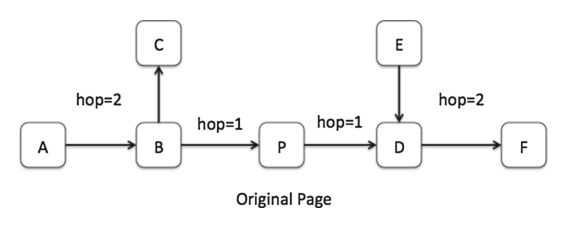
\includegraphics[scale=0.95]{Figures/GenreSim_Draw.eps}
		\caption{A directed graph of  web-pages \parencite{zhu2016exploiting}.}
		\label{fig:GenreSim_Draw}
	\end{center}
\end{figure}

\textit{GenreSim} is a ranking algorithm based on \textit{PageSim} algorithm, extended to fit in the problem of WGI. Similar to all this kind of algorithms, is based on the assumption that the more web-pages referred to a particular page, the more this page is related to them with respect to topic and/or genre. As concerns genre class, GenreSim focuses on \textit{forward} $F(p)$ and \textit{backwards} $B(p)$ hyperlinks. Moreover, utilizing the entire graph structure, web-pages are characterized as \textit{Hubs} $H(p)$ or \textit{Authorities} $A(p)$. The null hypothesis of the algorithm is that the web pages of the same genre are inter-connected with their hyperlinks. Consequently, a few pages backwards and forwards to a specific web-page compose a small network of the same genre. Using this "genre-network", the textual (and partially the structural) information of neighbouring web-pages can be used to amplify the signals required to classify a new web-page to that genre.

In more detail, hubs are pages with many outgoing hyperlinks, whereas pages with many incoming hyperlinks are called authorities. The number of incoming and outgoing hyperlinks are increasing the respective scores as shown in equation \ref{eq:GenreSim_hub_authortities}. However, web-pages with high score but with few backward hyperlinks are quite likely to be \textit{spam} pages. In order to regulate this, the $\omega(p)$ factor is introduced in equation \ref{eq:GenreSim_omega}, to reduce the score for the web pages with few backward hyperlinks. In addition, this is also useful to normalize the few links issue. That is, the number of the backward links is correlated to the number of links the page itself contains. 

\begin{equation}\label{eq:GenreSim_hub_authortities}
	\begin{array}{l}
		H(p) = \sum_{u \in V|p \to u} \omega(p) A(u) \\  
    	A(p) = \sum_{v \in V|v \to v} \omega(p) H(u) \\
    \end{array}
\end{equation}
\begin{equation}\label{eq:GenreSim_omega}
	\omega(p) = \frac{N}{|\log N - \log N(p) | + 1} 
\end{equation}

Therefore, the score for a new web-page in a given $G$ graph of web-pages, is calculated by equation \ref{eq:GenreSim_Score}. In general, the genre-selection recommendation score is propagated to the graph path $P(u,v)$ as indicated by the $Score(u, v)$ function of equation \ref{eq:GenreSim_Path}. Therefore, the score of a recommended web-page is decreasing gradually as this pages lies away (in hops) from the web-page to be classified. The $d$ factor is set to be $0.5$, i.e. the page score is decreasing by half for every hop away from the page under examination (see Figure \ref{fiig:GenreSim_Draw}). 

\begin{equation}\label{eq:GenreSim_Score}
	Score(p) = H(p) + A(p)
\end{equation}

\begin{equation}\label{eq:GenreSim_Path}
	Score(u, v) =
      \begin{cases}
      	\sum_{p \in P(u, v)} \frac{d Score(u)}{\prod_{x \in p, x  \neq v} (|F(x)| +|B(x)|)}, & v \neq u \\
        Score(u), & v = u \\ 
       \end{cases}
\end{equation}

Finally, the similarity of the candidate neighbour pages to the one under evaluation is based on the ratio of the min and the max path-score sums of all the possible paths, backwards and forwards, to the page under evaluation. This is defined as follows:

\begin{equation}\label{eq:GenreSim_Selection_Score}
	Sim(u, v) = \frac{\sum_{i=1}^{n} min(Score(v_{i}, u), Score(v_{i}, v))}{\sum_{i=1}^{n} man(Score(v_{i}, u), Score(v_{i}, v))}
\end{equation}

Hyperlinks themselves can be exploited by extracting information from the URL string and not from the hyperlink-graph. Particularly, a URL can be segmented to its components, i.e. the domain name, the path after the domain and the anchor text. Special characters such as $\{_ , . , ?, \$ , \%\}$, top-level domains $\{.gr , .uk , .com, etc\}$, and file suffixes such as ".html", ".pdf" are usually discarded and then character n-grams are extracted from the URL counterparts. 

WGI experiments using only the hyperlink information combined (or not) with other web-page information seems to be a promising researching path especially for performance oriented WGI applications such as genre-based focused-crawling where only the URLs are available \parencite{jebari2014pureURL,jebari2015combination,abramson2012_URL,priyatam2013don_URL} 
\textcolor{red}{(MSc reference on focused-genre-crawling)}

\subsection{Feature Weighting and Selection}

Term weighting is an essential issue in text mining applications. The features extracted from web-pages can be represented using a variety of  traditional weighting schemes such as Binary representation, Term Frequency (TF), and Term Frequency - Inverted Document Frequency (TF-IDF) \parentcite{sharoff2010web,santini2007automatic}. 

The binary scheme is the simplest and according to which each term is represented by a binary value indicating its occurrence or absence in the document. Despite its naivety, very good results were obtained using this scheme in WGI studies \patentcite{kanaris2009learning,sharoff2010web}.

TF weighs each term according to its frequency in the document. Several variations of this approach can be found in the literature. For example, the raw frequency of terms can be used. This certainly depends on the length of documents. Another idea is to normalize the raw frequency of a term over text length:

\begin{equation}
    TF(t,d) = \frac{f(t,d)}{length(d)}
\end{equation}

\nointend where $f(t,d)$ is the raw frequency of term $t$ in document $d$. Yet another modification is to divide the raw frequency with the maximum frequency of any term in document $d$.

TF-IDF is a balancing weighting scheme of document terms (e.g., word n-grams, character n-grams, POS n-grams, etc) given a collection of documents. It regulates the significance of the very low and very high frequency terms of the collection. That is, it decreases the value of the very high frequency terms (i.e., function words), and increases the importance of very low frequency terms when they occur in only a few documents. The calculation of a terms IDF in a documents collection is shown in equation \ref{chap:relevant_work:eq:idf}
 
 \begin{equation}\label{chap:relevant_work:eq:idf}
 	IDF(t) = log \left( \frac{N}{df(t)} \right)
 \end{equation}
\noindent
where $N$ is the number of the documents in the collection and $df(t)$ is the \textit{document frequency} of $t$, that is the number of distinct documents it occurs. 

Although TF-IDF is a popular choice in many text mining studies, the study of \parencite{sugiyanto2014term} demonstrates that it is not the best choice for WGI tasks. On the contrary, they propose a genre-specific weighting scheme, called TF-IGF. 
 
The main idea is that instead of considering a collection of documents, they consider a collection of genres (i.e., each genre is a collection of documents). Then, the terms are weighted by using the frequency of the term within a genre and the \textit{genre frequency} of the term (i.e., the number of different genres it occurs). :

 \begin{equation}\label{chap:relevant_work:eq:tf_igf}
 	TF-IGF(g,t) = f(t,g) \cdot (1 + log \left( \frac{N}{gf(t)} \right)
 \end{equation}
\noindent
where $f(t,g)$ is the frequency of term $t$ in genre $g$ and $gf(t)$ is the genre frequency of $t$. Since TF-IGF depends on genre, the average value over all genres in a given palette is finally used. The TF-IGF score can be used to select the most informative features that highlight genre-related information and reported results show that it is a better criterion for feature selection in comparison to regular TF-IDF \parencite{sugiyanto2014term}.

In \parencite{kanaris2009learning} a frequency-based method to select the most promising features is described. Initially, the feature set comprises character n-grams of variable length ($n = \{3, 4, 5}$. Then the \textit{LocalMaxs} algorithm is used to find the most prominent n-grams taking into account the frequencies of constituent n-grams of lower order (using a \textit{glue} function). The reported results show that this simple approach is quite effective in WGI tasks.

Another WGI-specific term weighting scheme has been suggested to deal with features obtained from URLs of web-pages \parentcite{jebari2014pureURL}. In particular, an approach called \textit{Structure-oriented Weighting Technique} (SWT) first extracts character n-grams from URLs and then each n-gram is weighted according to the following: 

\begin{equation}\label{eq:jebary_url_weigh_cngrams_1}
	SWT(t, d) = \sum_{s} w(s) f(t, s, d)
\end{equation}

\noindent
where $f(t,s,d)$ denotes the raw frequency of n-gram $t$ in section $s$ of document (i.e., URL) $d$. Namely, this approach assumes that the URL is segmented into fields and each field has its own importance, as follows:

\begin{equation}\label{eq:jebary_url_weigh_cngrams_2}
	w(s) = \left\{
    	\begin{array}{lll}
        	\alpha & if & s = Domain\ Name \\
            \beta & if & s = Document path \\
            \gamma & if & s = Document name \\
         \end{array}
  \right.
\end{equation}

Weights $\{\alpha,\beta,\gamma\}$ should be defined empirically using a training corpus \parentcite{jebari2014pureURL}. 

\textcolor{red}{THERE IS NO REFERENCE FOR THE FOLLOWING WORK. IN ADDITION THE FORMULAS SEEM PROBLEMATIC AND NOT WELL DEFINED}

Another genre-specific term weighting approach has been proposed for the task of video genre detection where textual information such as subtitles and brief descriptions are used. In websites like IMDB and Movelens it is also possible for the the users to create their own tags in addition to the existing keywords manually created by human experts. These user-created tags can be exploited in a similar manner as the words of the subtitle text for classification of the video to their genre. Particularly, it has been shown that the user tags provide a rich source of information and enhance performance of genre detection in comparison to the case only keywords are used. In order to appropriately estimate the importance of user tags a fuzzy extension of TF-IDF weighting scheme is introduced.

Although the above method was aiming for building an effective recommendation system here it is presented briefly for the innovative weighting scheme which is exploiting the meta-data of the tags. Particularly the aforementioned user tags are in fact triplets of  $\{Tag, Movie, User \}$. The idea is to exploit the frequency of users selecting a tag for a movie and then the number of different movies a tag has been assigned to, similar to TF and IDF factors.

To do so, initially the \textit{Appropriateness} of a tag is estimated by counting the number of times users assigns the same tag to a movie that belongs to a specific genre as follows:

\begin{equation}\label{chap:relevant_work:eq:fuzzy_movies_genre_eq1}
	tf_(u_{j},g_{i}) = \frac{\sum_{m \in G} tagged(t,u,m) }{ \max_{t \in T} \sum_{m \in G} tagged(t,u,m)}
\end{equation}
where $tagged(t,u,m)$ is 1 when a user $u$ tag with t the movie $m$ when it belongs to genre $g$, and $0$ if not. The score of a tag similar to the TF-IDF is called Degree $deg(t,m,g_{i})$and it is the weighted frequency of users as singed this tag by the \textit{Importance Score} $imp(t,g_{i})$ of the tag, as shown in equation \ref{chap:relevant_work:eq:fuzzy_movies_genre_eq2}

\begin{equation}\label{chap:relevant_work:eq:fuzzy_movies_genre_eq2}
	deg(t,m,g_{i}) = uf(t,m) \cdot imp(t,g_{i})
\end{equation}
Where $uf(t,m)$ is the frequency of the users assigned the this tag to a movie $m$. The $imp()$ is calculated by the \textit{Fussy Linguistic Ordered Weighted Averaging Aggregation Operator (OWA)} of the equation \ref{chap:relevant_work:eq:fuzzy_movies_genre_eq1} weighted by the \textit{Uniqueness} of the tag. The uniqueness is also the OWA compliment of the term among all the genres of the taxonomy. The $imp()$ is then calculated by the equations \ref{chap:relevant_work:eq:fuzzy_movies_genre_eq4} and \ref{chap:relevant_work:eq:fuzzy_movies_genre_eq4}.

\begin{equation}\label{chap:relevant_work:eq:fuzzy_movies_genre_eq3}
	t_{most}(g_{i}) = \oint_{j=1}^{U} tf_(u_{j},g_{i})
\end{equation}

\begin{equation}\label{chap:relevant_work:eq:fuzzy_movies_genre_eq4}
	imp(t,g_{i}) = \oint_{j=1}^{U} tf_(u_{j},g_{i}) \cdot (1 -  \oint_{i=1}^{G} t_{most}(g_{i}))
\end{equation}

Where $\oint=OWA$,  $g_{i}$ is a particular genre, $G$ is the number of the genres in the taxonomy and $U$ is the number of users used this tag for this genre.

Finally, for the movie genre categorization a binary vector of the genres list is returned of the \textit{Quantised  $\max_{t \in T} deg()$}. The maximum degree values of the genre tag is set to $1$ when it is above the \textit{mean values of all tag-degrees} and zero otherwise.


%\subsection{Dimensionality Reduction}

%In most of the applied research domains where machine learning is the dominant subject of choice the main concern is to extract and select the proper features from the raw data samples of the data set. Therefore, in addition to the process of inverting a machine learning method for inducing prediction models for the problem the process of feature extraction and dimensionality reduction are coming together. The same applies for the WGI where most of the focus where in these two procedures and less in creating new machine learning algorithms. On the contrary, in all studies usually a closed-set and out-of-the-box ML models were tested with the exception of the cases described in sections \ref{chap:relevant_work:sec:machine_learning_methods} and \ref{chap:relevant_work:sec:openset_and_noise}.

%In this section are summarized all feature selection and dimentionality reduction successful ideas for WGI and AGI. To begin with the features that can be extracted from a web-pages can be grouped to the \textit{textual}, the \textit{HTML tags} and the \textit{URL links} with or without their \textit{anchor text}. Cornering the URL links it will be discussed in more detail in section \ref{chap:relevant_work:sec:url} where either the URL it self as a character string can be analyzed or the structure of the web-pages connections can be exploited \parencite{abramson2012_URL,asheghi2014semi,jebari2014pureURL,priyatam2013don_URL,zhu2011enhance}. 

%Usually, the combination of features from different sources enhances the robustness of WGI approaches \parencite{levering2008using,kanaris2009learning}. However, features extracted from textual content are more robust since they do not  depend on technology or format used to create a web page and therefore they are more likely to remain constant in time given that the W3C is changing the specification of the HTML regularly, for covering the occurring needs. This is the reason that this work is only focusing on the textual information in the next chapters.

%Although the improvement was impressive by just changing the weighting schema, especially for  the size of the vector space, one should consider that the experimental set-up was only for the closed-set scenario. Moreover, the TF-IGF similarly to the TF-IDF is tightly related to the collection itself, therefore, the results closely are related to the 7-Genres collection. Given that these collection are old and the nature of the highly temporal idiosyncrasy of the genre-taxonomies, it is high likely this method to have high bias. On the other hand in closed-set cases where the texts collection is constrained considering documents number (i.e. slowly expanding) and genre-taxonomy size (i.e. rarely updated) the TF-IGF seems to be efficient, and with very low computational cost.  

%Dimentionality reduction and the \textit{selected features encoding in to a multi-dimensional vector} is an important aspect concerns the WGI research. As aforementioned \textit{features selection} implicitly affects the compression of the vector space, however, there are other explicit methods than have been tested for WGI.

%BOT and TF-IDF approaches seems to work almost as good as more complex features such as POS, $\chi^{2}$ statisics etc. However, in some cases explained before such as Wikipedia, blogs, news sub-genre the complex features (and heuristics) seems to work better. It seems that is is the result of the implicit dimentionality reduction which enables an ML model to be optimized in a more informative vector space.

%Although, the above statement might be a subject of a great research arguments, what we unsuitably know is that in a smaller and more informational dense vector space a ML algorithm will perform much better with great certainty. Thus, a method that could potentially reduce the vector space and manage to encode the maximum of the required information, it would at least improve significantly the speed performance of any ML algorithm. 

%In order to make an intuition about the "curse of dimensionality"  and on how the feature selection can encode more information in case dimensionality reduction, a mind experiment is presented bellow. 

%Lets assume task where a ML model should be trained in a multi-class classification task for the whole genre-taxonomy of the WWW and assuming that all the genre of the Web where idd and known. In that case the whole Oxford Dictionary would have defining the vector space of the problem. 

%The Oxford dictionary English is containing $171,476$ words thus the vector space would have been very sparse. The amount words can be calculated also by using the Combinatorial Calculation using the \textit{binomial coefficient} minus the invalid combinations, of the $26$ English letters (assuming the the whole Web was only written in English language), as shown in equation \ref{chap:relevant_work:eq:en_vocab_size_calc}.

%\begin{equation}\label{chap:relevant_work:eq:en_vocab_size_calc}
%	 \left(
%    	\begin{array}{c}
%        	n = 26\\
%            k = 1\\
%         \end{array}
%	\right)
%    +
%    \left(
%    	\begin{array}{c}
%        	n = 26\\
%            k = 2\\
%         \end{array}
%	\right) 
%    +
%     \cdots 
%    +
%   \left(
%    	\begin{array}{c}
%        	n = 26\\
%            k = Max Eng. Word\\
%         \end{array}
%	\right) 
%    = 300,430 - \{Invalid Combinat.\} =  171,476
%\end{equation}
%On the other hand if we are using the Character n-grams of size $3$ (C3G) or $4$ (C4G) then for C3G the vector space is $2600$ \textit{minus the set of invalid combinations} and for C4G becomes $14950$. As we also know from the literature and it will presented later in this study the CNG features are returning the highest score in WGI ML modeling. Moreover, the \textit{character tuples} are capturing stylistic properties of the texts, where it is an information which is lost when it is "hidden" in the words.

%To conclude, dimentionality reduction is the main objective in the process of feature selection and as explained so far there are several heuristics than can applied to achieve this. There cases where a terms (word or char, n-gram) is selected only when it can be counted in more than a specific number of web-pages in a corpus. Moreover, there are cases where only the words above a specific threshold are selected, usually the length varies from 2 to 5 characters length. In addition is has been shown that \textit{Stop words} (Stamatatos) and 
%\textit{Surface cues} (Kessler) from the superficial document metrics are important and some time better (and lighter in terms of speed in model training) than the raw BOT. 

%All the aforementioned approaches is a implicit method for dimentionality reduction and documents information encoding. However, \textit{Graph based features} is an explicit method for this and usually is applied after them feature selection process.

\section{Machine Learning Approaches to Genre Identification}
\label{chap:relevant_work:sec:machine_learning_methods}

Genre identification of documents is generally viewed as a text categorization task. After defining a feature space to represent documents, a classification algorithm can be applied to a training set in order to learn to distinguish between genres. As already pointed out, the majority of previous work studies consider this to be a closed-set classification task. In addition, most of the existing studies consider a flat genre palette where each genre is independent on the other genres. In the remaining of this section, the machine learning algorithms that have been used to learn the properties of genres are discussed according to the adopted setup of the task. 

\subsection{Closed-set Genre Recognition}

The main research volume in this area adopt a closed-set classification framework. Several well-known machine learning algorithms have been used for this task, including SVM, Naive Bayes, Random Forest, Decision Trees, Ensemble-based models \parencite{Lim2005,santini2007automatic,kanaris2009learning,jebari2015combination,sharoff2010web}. 

The SVM classifier was tested either in binary or multi-class WGI tasks \parencite{dai2018fine}. It is an algorithm than can easily handle high-dimensional and sparse feature spaces \parencite{joachims1997probabilistic}. In \parentcite{sharoff2010web} analytical experiments using a variety of datasets demonstrated that SVM WGI models could surpass the best reported results in most of the cases combined with character n-gram features. In addition \parencite{virik2017blog} compare SVM models with Naive Bayes and k-Nearest Neighbours models on the recognition of Blog sub-genres. The reported results show that SVM obtained higher accuracy results. Recently, an SVM-based approach was tested on the very challenging case of cross-Lingual genre classification (i.e., when the training documents are in one language and the test documents in another language) and obtained very promising results \parencite{nguyen2019cross}. 

Distance-based approaches in the WGI task include mainly variations of nearest-neighbor classifiers. One particular case is based on ranked feature distributions distances \parencite{waltinger2010feature}. The features of the samples of a class are ranked in descending order according to their TF or TF-IDF values. In order to measure the distance of a new web-page from the classes, the features of the new web-page are also ranked and then the difference in rankings indicate the most similar class. That is the TF or TF-IDF value of features is not important anymore since only the ranking of features is considered. Moreover, when a feature is not present in either the new web-page or a class, then a predefined $Max$ value is assigned. The total \textit{ranking distance} between a web-page $d$ and a class $g$ is calculated as follows:

\begin{equation}\label{eq:ranking_distance}
	d(d,g,t) =
      \begin{cases}
      	| r_{d}(t) - r_{g}(t) |, t \in d \wedge t \in g  \\
        Max, t \notin d \vee t \notin g \\ 
       \end{cases}
\end{equation}

\begin{equation}\label{eq:ranking_distance_sum}
	rd(d,g) = \sum_{t} d(d,g,t)
\end{equation}

The new web-page is then classified to the nearest class. The accuracy of this method has been reported to surpass that of SVM using the same features \parencite{waltinger2010feature}.

Following the impressive performance obtained in classification tasks involving natural lanaguage texts, deep learning algorithms have also been tested in WGI tasks \parencite{strobel2018text}. A \textit{recurrent neural network} comprising 200 gated recurrent unit cells in the hidden layer. On top of that, a fully-connected layer assigns documents to classes using a Softmax decision function. Very promising results are reported for this deep learning model in closed-set WGI tasks.

Instead of learning a simple model, ensemble methods attempt to extract several base models and then combine them. One main direction is to use well-known ensemble learning methods such as AdaBoost, Bagging and Random Forests \parencite{sugiyanto2014term,onan2018ensemble}. This approach can easily handle high-dimensional representations and heterogeneous features.

\textcolor{red}{Although, the traditional bag-of-words approach had better result with XABoost or other techniques been tested for over a decade on genre identification or/and particularly on WGI, distributional feature models are early showing their advantages over the TF-IDF (or TF alone) models[REF].}

%\paragraph{Random Forest} Several studies among other classification algorithm they have extensively used \textit{Random Forest Classifiers}. Usually they use this algorithm in an out-of-the-box format. Most importantly seem to be one of the high score performance algorithms and most of the time the best solution. Although, most the studies are focusing of features selection/extraction and the term weighting schemes one could reason the high performance of the Random Forests to its internal ability to selecting the internal connection of the  features which \textit{resembles the word embedding} (FIND REF FOR THIS ARGUMENT) \parencite{sugiyanto2014term}

Another idea is to build a separate model for each web-page modality. For example, an ensemble algorithm called \textit{Multiple Classifier Combination} (MCC) is presented in \parentcite{zhu2016exploiting}. Particularly, the main idea is use information from a web-pages to be classified to a given genre palette as well as information from a set of neighbouring web-pages (i.e., that are near the specific web-page in the graph formed by hyperlinks between pages). The MCC algorithm builds a set of SVM classifiers each trained using a particular set of features. Then a decision matrix is formed including all predictions of base SVM classifiers:

\begin{equation}\label{chap:relevant_work:eq:GenreSim_DP}
	DP(p) = \left(
    	\begin{array}{ccc}
        	d_{11} (p) & \cdots & d_{1|G|} (p) \\
            d_{21} (p) & \cdots  & d_{2|G|} (p) \\
            & \vdots & \\
            d_{N1} (p) & \cdots  & d_{N|G|} (p) \\
         \end{array}
\right)
\end{equation}

\noindent
where $d_{ij}$ is the membership degree given by classifier $i$ to genre $j$, $N$ is the number of base classifiers, and $|G|$ is the number of genres. Then, the final decision is taken by applying simple methods to combine these predictions columnwise, such as the min, max or average rules.

%\textit{AdaBoost} is a \textit{Boosting} algorithm where usually a random sampling is performed over the data and s set of classifier are trained over these samples. There is a weighting scheme over the samples which is changing in every training iteratio, where for the samples mostly miss-classified, by most of the learners, their weights are increasing. In this manner the difficult samples repetitively to classification are presented to the weak learner in more iteratios in order the whole systems of learners fit adjust better over these samples.

%\textit{Bagging/Bootstrap aggregating} is an ensemble learning methods where a set of independent learners are training on different subsets of samples. Sampling with replacement is employed for Bagging, usually random. The performance of the ensemble is significantly influenced by the sampling policy/model. The ensembles decision is obtained either by the majority voting or my the weighted voting for a random sample.

Another \textit{late fusion} ensemble is proposed in \parencite{finn2006learning}. Again, the idea is to build homogeneous base models each trained only on a specific feature subset. In the testing phase the majority voting us a common strategy. Particularly in their study they learn C4.5 decision trees for different web-page modalities (i.e., BOW, POS, text statistics features) and then build a \textit{Multi View Ensemble} that combines the predictions of the modality-specific models. It is important to note that in the training phase \textit{Active Learning} was used. This is a sample selection strategy where an an evaluating process was indicating which sample was better to be used for the specific C4.5 learner, for a given feature set. The late fusion ensemble with the active learning strategy obtained promising results including the domain transfer scenario.

\subsection{Open-set Classification}
\label{chap:relevant_work:sec:openset_and_noise}

Most previous studies in WGI consider the case where all web pages should belong to a predefined taxonomy of genres \parencite{Lim2005,santini2007automatic,kanaris2009learning,jebari2014pureURL}. This corresponds to the closed world assumption. However, this naïve assumption is not appropriate for most applications related to WGI since it is not possible to construct a universal genre palette that covers at least a great extend of the Web. Web-pages that do not belong to any of the predefined genres are considered noise and also include web-pages where multiple genres co-exist \parencite{santini2011cross,levering2008using}. 

Noise in WGI can be categorized into structured noise and  unstructured noise. The former assumes that there is no information about the composition of noise (i.e., a random collection of web-pages not belonging to the known genres) \parencite{santini2011cross}. The latter assumes that noise is composed by several unknown genres (i.e., for which there are no training examples). However, it is highly unlikely that such a collection  represents the real distribution of pages on the web.

The effect of noise in WGI  was first studied in \parencite{shepherd2004cybergenre,kennedy2005automatic} where predefined genres were personal, organizational, and corporate home pages while noise consisted of non-home pages. However, the distribution of pages into these four categories was practically balanced, hence it was not realistic. In another study, a clustering framework is used where one cluster is built for each predefined class and another cluster is built for the noise \parencite{kennedy2005automatic}. 

To handle noise in WGI there are two options. First, to adopt the closed-set classification setup having one predefined category devoted to noise. That is training examples for known classes as well as the noise class are provided. Since this category would comprise all web pages not belonging to the known genre labels, it would not be homogeneous. Moreover, this noise class would be much more greater with respect to the other genres causing class imbalance problems. 

A few studies follow this direction. In these cases samples of noise is available in the training phase of the prediction model. In \parencite{Vidulin2007} structured noise samples constitute the negative class of a binary classifier. The most common approach to handle noise is to build binary classifiers where the positive class is based on a certain predefined category and the negative class is based on the concatenation of
all other predefined categories plus the noise \parentcite{kennedy2005automatic}. In \parentcite{dong2006binary}
noise is used as the majority class in an experiment where 190 instances from personal homepage, FAQ, and e-shop categories were used in combination with 600 noise pages. Similarly, \parentcite{levering2008using} use about 200 instances for the predefined genres of store homepages, product lists, and product descriptions in combination with about 800 other pages (noise). Such a combination of binary classifiers can also be seen as a multi-label and open-set classification model where a web page can belong to different genres and it is possible for one page not to belong to any of the predefined genres. From another point of view, \parentcite{jebari2015combination} considers outlier samples of known genre labels as noise and excludes them from computing the centroids that represent genres in mult-label WGI. The centroid of a genre is then adjusted each time a new web page is classified to that genre. 

Another, more realistic option is to adopt the pore open-set classification setting where training examples belong only to known classes and it is possible for some web pages not to be classified into any of the predefined genre categories. This setup avoids the problem of class imbalance caused by numerous noisy pages and also avoids the problem of handling a diverse and highly heterogeneous class. On the other hand, open-set classification requires strong generalization with respect to the closed-set setup. A more concrete open-set classification models for WGI is presented in \parencite{stubbe2007genre}. However, this model was only tested in noise-free corpora. Nevertheless it has been shown that it is much more challenging to perform WGI in the noisy web in comparison to noise-free corpora \parencite{Asheghi2015}.

\textcolor{red}{DESCRIBE IN DETAIL SCHEIRER-2013 and ASHEGHI-2015 OPEN SET APPROACHES}

Another open-set classifier is presented in \parencite{chen2012genre}. It is an ensemble approach composed by two base SVM classifiers each trained using a different mutually exclusive training subset. The assumption of this approach is that part of the support vectors will be optimized for every SVM preserving the generalization of the two independent models and the combined classification will manage to fit well over the whole corpus. The combination of the output of the base models is a pairwise genre operation that examines whether the SVM classifiers agreee on their decision about a new web-page:

\begin{equation}\label{eq:office_doc_ensemble}
	(g^{k}_{1}[i] \vee g^{k}_{2}[i])  \wedge  (g^{m}_{1}[i] \vee g^{m}_{2}[i]) ,   \forall m \neq k
\end{equation}

where $\{k, m\}$ are the genre classes and $\{g_{1}, g_{2}\}$, are the SVM classifiers. For any new web-page, the truth table of this binary rule for all genre pairs might end up full of zero values. Then, this page remains unclassified. In all other cases at least one genre will return as true. 
		
The above ensemble is an early fusion approach where the different features and document representations are all combined in a concatenated vector for each document. Then the concatenated vectors are the input for the learners of the ensemble.

%Another recent approach related to the open-set classification on the \textit{Text Classification} problem was suggesting the reduction of the \textit{open space risk} using an SVM based methodology. Particularly, they are comparing eight (8) SVM based methods (additionally with an EM Semi-supervised method) in a open-set setup. They have compared their method with an  SVM center-based similarity space learning methods and some other methods, also in a open-set setup. Their method outperformed the others significantly, with some exceptions. 

%Their main contribution is the transitions of the problem form the \textit{feature space} to the \textit{distance space}. Particularly they are using ten (10) different centroids one for each of the five (5) different distance measures proposed by (Fei and Liu 2015......) and for two (2) different document representations one for uni-grams and one for bi-grams. Their centroids are calculated using  eq \ref{eq:manning_centroids} 

%\begin{equation}\label{eq:manning_centroids}
%	c_{j} = \frac{\alpha}{\lvert D_{+} \rvert} \sum_{d_{i} \in D_{+}} \frac{x_{j}^{i}}{\lVert x_{j}^{i} \rVert } - \frac{\beta}{\lvert D - D_{+} \rvert} \sum_{d_{j} \in D - D_{+}} \frac{x_{i}^{j}}{\lVert x_{i}^{j} \rVert}
%\end{equation}

%where $D_{+}$ is the set of documents in the positive class and $\lvert . \rvert$ is the size of function. $\alpha$ and $\beta$ are parameters, which are usually set empirically.

%The SVM methods under testing where 1-vs-rest multi-class SVM (Platt200...), 1-vs-set Machine SVM \parencite{scheirer2013toward}, W-SVM (Scheirer2014....), $P_{1}$-SVM (Jain2014), $P_{1}$-SVM (Jain2014), Exploratory Seeded K-means (Exploratory EM) (Dalvi2013...). They have also used a kind of \textit{openness testing}, by using $25\%$ to $100\%$ of the classes and their method were mostly outperforming the other methods. The macro-F1 score range of their methods from the most open set-up to the totally closed (i.e. using the $100\%$ of the classes) was from $0.417$ to $0.873$ depending on the corpus and the special class set-up \parencite{fei2016breaking}.

%To sum up, as concerns the classification models involved in WGI studies, when a given genre taxonomy is utilized and there is no noise, then well-known machine learning models, like SVMs, decision trees, neural networks, naive Bayes, Random Forests, etc. are used \parencite{Lim2005,santini2007automatic,kanaris2009learning,jebari2015combination,sharoff2010web}. In case of presence of noise, in a clustering framework described in \parencite{kennedy2005automatic} one cluster is built for each predefined class and another cluster is built for the noise. However, the most common approach to handle noise is to build binary classifiers where the positive class is based on a certain predefined category and the negative class is based on the concatenation of all other predefined categories plus the noise \parencite{kennedy2005automatic,dong2006binary,levering2008using}. Such a combination of binary classifiers can also be seen as a multi-label and open-set classification model where a web page can belong to different genres and it is possible for one page not to belong to any of the predefined genres. 

\subsection{Semi-supervised Learning} 

In WGI, there is lack of large labeled corpora including multiple genres and sufficient training samples per genre. On the other hand, there is plenty of unlabeled examples that can easily be used. One suggested direction in WGI research is the use of \textit{semi-supervised learning} approaches in order to exploit the virtually infinite number of unlabeled data of the Web. 

Particularly, in \parencite{chetry2011web} the \textit{Co-Training} algorithm is used. Their model is based on a SVM and a Naive Bayes classifier trained on $1,232$ labeled web-pages as well as a set of $20,000$ unlabeled samples. Co-Training is based on an iterative process where the unlabeled data are classified by the classifiers initially trained using the labeled data. In every iteration the highest ranked unlabeled samples, in terms of classification certainty of the classifiers, are labeled accordingly and the training of classifiers restart using these new samples together with the previously labeled samples. The process continues until all unlabeled samples have been used or a specific number of iterations is reached. The reported results show an improvement in performance over a regular SVM classifier. The experiments were set on a closed-set framework with a corpus including the genres of \textit{Spam, Discussion, Educational Research, News Editorial, Commercial, Personal Leisure}.

Domain transfer is the ability to learn a model using training examples from one domain and be robust enough to be applied to another domain. As an example, for the genre News there might be several topic domains such as Sports, Technology, Science, Health, Politics. An ML model which has been trained for News only on Sports topic and still can perform equally well for Technology, etc, it considered robust. This is very important particularly for genre identification tasks where usually the positive available samples for a genre do not cover a wide range of topics. An extreme case of domain transfer is cross-Lingual genre classification where the task is to train a model using documents in one language and then apply the model to documents in another language, particularly with different linguistic properties, such as English to Chinese and vice versa.

One proposed solution to achieve robustness across domains is presented in \parencite{petrenz2011stable}. Their approach focuses on the use of language-independent features such as character-n-grams and surface text characteristics such as type/token ratio with an \textit{iterative strategy of training a ML model}. Such a method is the \textit{Iterative Target Language Adaption (ITLA)}. 

\textit{ITLA} a special case of cross-lingual AGI method where pair-wise inter-language training is possible. That is, one can train a model to one language and then optimize it to another. This method enables the potential training of a model on one language and adapted to another with few labeled samples set for the required genre taxonomy and a rich set of unlabeled samples. In \parencite{petrenz2011stable} SVM was the model of choice. The process includes the following steps:

\begin{enumerate}
\item Initially train an SVM classifier on language $L^{L}_{S}$. Then with the help of unlabeled $L^{U}_{T}$ set for the target language the model is evaluated for its prediction confidence on the genre taxonomy.
\item Using a labeled subset of the target language set $L^{L}_{T}$, another SVM model is trained where the prediction confidence of the initial training is used for selecting only the samples of the subset returning the highest confidence score. 
\item The samples with very low score in $L^{L}_{T}$ are filtered out and a new subset is re-sampled.
\item The process continues between the steps 2 and 3 until no change in the prediction confidence occurs or the iteration number has reached its pre-defined limit.
\end{enumerate}

The results in this study were very promising given that with a generic language independent approach manages to exceed the results of the common solution of using machine translation technology (i.e., where the texts of the  source language, used to train the model, are automatically translated to the target language and they are used to train the classification model).

\subsection{Hierarchical Classification} 

So far, all discussed methods assume that the genre palette consists of independent genres in a flat structure. Another approach is to consider a hierarchical structure of genres where super-genres and sub-genres are defined. Such a hierarchy can be obtained by human-experts.

An automated approach to build a hierarchy of genres is presented in \parencite{madjarov2015web}. First, they use two clustering methods attempting to develop an automated hierarchical clustering where a flat multi-class taxonomy could potentially be organized in a hierarchical structure. That is, given a set of  leaf class-tags, an agglomerative or a balanced \textit{k-means} algorithm is used to create a class hierarchy. 

The reported results show than balanced k-means works better for this task on their data set and experimental set-up. The success of balanced k-means can be explained by the fact that it needs the size of the clusters to be provided. Thus, the objective function of this method is to optimize two (contradictory) objectives: first, to find the most dense and well separated clusters and second to maintain the sizes of the clusters equal. To do so, the \textit{Hungarian} algorithm is used for the optimization process, a combinatorial optimization algorithm that solves the assignment problem in polynomial time.

The automatically obtained hierarchy has been compared with the one of built by a human-expert. The former has been found to work equally or even better than the latter. It has also been demonstrated that the obtained hierarchical structure can be used for a multi-class classification scenario \parencite{malinen2014balanced}. 

\subsection{Web Genre Temporal Property}
\label{chap:relevant_work:sec:temporal_wgi}
The temporal idiosyncrasy of the genre-taxonomy is a major factor, yet not deeply studied in the linguistics and computational linguistic domains. Naturally, as in other human arts there is an evolution in the genres, while other genres emerging and others stop existing. Web-genre taxonomy is a result of an even more dynamic environment and it evolves rapidly. Genres are adapting due to the medium transition such as from \textit{News on paper} to \textit{News on the Web}, or because of the medium itself emerging novelties such as the \textit{Blogs} which have evolved to\textit{ micro-Blogs} and finally to \textit{the Social-Media}. 

In \parencite{caple2017genre} there is a characteristic study advocating in the temporal manner of the web-genre, where it is analyzed how the News (as a web-genre) have changed overtime and the way the News sub-genres occurred.

An \textit{Enhanced Centroid-based Classification (ECC)} ensemble model has been proposed for dealing with adapted genres and the temporal idiosyncrasy of the genre-taxonomy. The model is an \textit{incremental centroid-based} ensemble where new web pages are classified one by one, where in the testing/production phase the centroids adjust to the new data as long as they are "close-enough" \parencite{jebari2015combination}.

The ECC learning algorithm is calculating an initial set of centroids for every given class based on the equation \ref{eq:jebary_ecc_centroids} and then using the threshold calculated by the equation \ref{eq:jebary_ecc_theshold} is re-evaluating the samples. When the samples of  class are not "close-enough" are considered to be \textit{outages} and a new centroid is calculated from the rest of the samples for this class. 

\begin{equation}\label{eq:jebary_ecc_centroids}
	GC_{i}^{N} = \frac{GC^{S}_{i}}{\Vert GC^{S}_{i}\Vert }
\end{equation}

\begin{equation}\label{eq:jebary_ecc_theshold}
	\sigma_{i} = \frac{1}{\vert g_{i} \vert } \sum_{p_{j} \in T_{r_{g_{i}}}} sim(p_{j}, GC_{i}^{N})
\end{equation}
\noindent
where $GC^{S}_{i} \in G$ is a set of predefined genre centroids for the $S_{i} \in G$ set of samples for each genre class $G$. $T_{r_{g_{i}}} =   \{ (p_{i}, g_{j}) \vert g_{i} \in G  \}$ is a set of training set samples initially and at the and is formed to $T_{r_{g_{i}}} =   \{ (p_{i}, g_{j}) \vert sim(p_{j}, GC^{N}_{i}) \leq \sigma_{i} \}$  after eq. will be applied \ref{eq:jebary_ecc_theshold}.

In the testing phase an arbitrary page is ranked in deciding order to the \textit{similarity-rank} $\theta(p)$, as defined in the equation \ref{eq:jebary_ecc_rank}. Then the centroids and the threshold are re-calculated based on the equations \ref{eq:jebary_ecc_new_centr} and \ref{eq:jebary_ecc_new_thres}. 

\begin{equation}\label{eq:jebary_ecc_rank}
	\theta_{i} = \{g_{i}, sim(p, GC_{i}^{N}) > \sigma_{i}\}
\end{equation}
\begin{equation}\label{eq:jebary_ecc_new_centr}
	GC_{i}^{N} =  \frac{GC^{S}_{i} + p}{\Vert GC^{S}_{i}  + p\Vert}
\end{equation}

\begin{equation}\label{eq:jebary_ecc_new_thres}
	\sigma_{i} = \frac{S_{i} +  sim(p, GC_{i}^{N})}{\vert g_{i} \vert}
\end{equation}
The ECC has been \textit{designed to adapt in the evolution of genres in time}, thus, it makes no sense to classify the web pages exclusively on the contrary is returning the similarly-rank $\theta(p)$. Consequently, this algorithm can be considered open-set \textit{because possible for same web-pages the  $\theta(p)$ set might return empty}. On the other hand since the algorithm will adapt some web-pages that are not strictly belonging to the genre it is trained for, i.e. noise pages, will be incorporated to the new centroids and the threshold value.  Consequently, ECC is sensitive to noise as it has been defined in section \ref{chap:relevant_work:sec:openset_and_noise}.


%\section{Web-Genres Identification using other than textual information}\label{chap:relevant_work:sec:intro}

\section{Deep Learning Vocabulary of Distributional Features for WGI}\label{chap:relevant_work:sec:word_embedding}

\textit{Distributional Features/Word Emending} based on the words or/and document encoding is the state-of-the-art in IR and NLP because it a practical solution for automatically modeling the process of feature selection, document representation and dimentionality reduction. This is the case for the AGI/ WGI tasks, and it is the second contribution to the domain together with the open-set approach.

In section \ref{chap:Document_Representation} and it is shown how a week ML algorithm can be trained with 100 times less features than the features given to an better algorithm for the WGI task. Moreover in section \ref{chap:relevant_work:sec:word_embedding} there is a discussion related to the word embedding and the \textit{Features Vocabulary Modeling}.


Given the complicated task of AGI, the traditional BOW models are unable to capture the enduring information span across sentences and paragraphs. Themes, registers and other properties of the texts cannot be captured only by the frequencies of the Terms (Word, Character, POS n-grams etc). The abstract concepts, the ontologies, the style and the form of the texts are only merely captured by a combination of heuristics as explained in section \ref{chap:relative_work:sec:heuristics}. 

The feature selection is so important that so far the simpler the model the better performs for the WGI task as long as the features are capturing \textit{the style and the concepts} of the texts. In \parencite{pritsos2019open}, which is part of this work, and also in \parencite{worsham2018genre} the \textit{Neural Language Modeling (NLM)} is proposed for the first time for WGI an AGI respectively. In both works the conclusion is similar. i.e. the ensemble based and boosting methods which are rather simpler than NLM are stile better performers on the task. However, in respect of speed performance and the automation in the process of feature selection the NLM seem to be the perspective research path for the following years.

Most proposed \textit{NLM} are designed to capture text in a sequential manner. That is, the model is encoding the meaning of the words based on the sequence of the previews terms (or following terms). Therefore, these models also called \textit{Distributional Models (DM)} and the NLM process is also called \textit{Word Emending}. The NNet models which have been tested are the \textit{Convolutional Neural Networks (CNN)}, the Recurrent Neural Networks (RNN), and the \textit{Long Short-Term Memory Networks (LSTM)}. 

The experimental procedures of this work is confirming the speed amplification in the WGI training and prediction process, mainly due to the dimentionality reduction and the better encoding of the abstract information required. However, it is also confirming that the process more the NLM was computationally expensive because of the length of the texts. In \parencite{worsham2018genre} there was an effort to reduce the problem and increase the performance of the NNet models.

Working with long pieces of text the NNet for example CNN the network is increasing as the data input is growing. On the other hand the RNN and the LSTM are sensitive to long sequences and their hyper-parameters are degenerated then they are becoming very slow in training for overcoming this issue. Moreover, to train these NNet models with long corpora is required a great hardware infrastructure. 

In order to reduce the training time and computational cost of the word-embedding modeling one can think of several strategies. It turns out that the best strategies is to use the \textit{All Chapters} training input. That is,  the training and the test set is splinted into chapters in a heuristic manner. Then the lengths of the chapters are normalized by getting only the $C_{Doc}$ length of the whole chapter, say the first 2,000 terms. In case the chapter is shorter the rest of the chapter is padded with an abstract term such as $\$pad\$$. 

As it has been reported the all-chapters strategy with a CNN returned $F_{1}=0761$ score which was the best of all the NNet combinations and features sizes. However, \textit{Random Forests} or \textit{XGBoost on sequential trees} and simple BOW, outperformed the NNet model with $F_{1}=0.79$ and $F_{1}=0.81$ respectively. XGBoost is a highly optimized, \textit{Gradient Boosting }solution which is made up of a boosted set of sequential trees learned from the gradients of some differentiable loss function\textbf{ (Chen and Guestrin, 2016).}

In \parencite{pritsos2019open} a work is presented where Doc2Vec has been used for the WGI task on KI04 corpus. Detail are discussed in section \ref{word_embedding}. It is shown that \textit{Distributional (DL) features} can make a weak open-set learning algorithm namely the \textit{Nearest Neighbour Distance ratio} classifier to a combative learner. When it come to comparison in the open-set framework with the RFSE, the NNDR seems performing lower, however, the size of the document vectors are 10 to 100 times smaller because of the DL features. 

In these experiments the whole KI04 corpus is given to the NNet document encoder. The line of thought is the same as Word2Vec and the word embedding, i.e. as an extension of the words encoding the documents can be encoded to a fixed size vector space. 


% ""Examples of word vectors include Word2Vec (Mikolov et al. 2013), GloVe (Pennington, Socher, and Manning 2014), Eigenwords (Dhillon, Foster,and Ungar 2015), and Fasttext (Bojanowski et al. 2017). These word vectors are usually referred to as distributional word vectors, as their training methods rely on the distributional hypothesis of semantics (Firth 1957)."""


The state-of-the-art in the text-genre classification and WGI is the Vocabulary-Learning and particularly the use of the deep-learning methods for building comprehensive word encoding vocabularies or document encoding. 

This methods due to the nature of the Neural-Networks, mainly used,  the procedure for building vocabulary models is \textit{implicitly embedding} a variate of information\textit{ syntactical, morphological and structural}. However, there are some efforts, where these kind of information was \textit{"explicitly encoded"} by using other methods inspired by signal processing and dimentionality or noise reduction techniques.


In \parencite{kim2010formulating} it is proposed the \textit{Harmonic Descriptor Representation (HDR)} of the web-pages inspired by the musical analogy of a string musical instrument. Then the document is consider to be a temporla sequence of signals, i.e. the characters or word n-grams. In similar manner to the NLE models it is captured explicitly the \textit{Distributional Properties} of the texts. Particularly instead of the terms occurrence counting the intervals of the the occurrences are measured, in addition the length of the documents are encoded and normalized implicitly. 

The HDR word encoding is a tuple of three explicit measurements; the FP, LP and AP. Moreover the \textit{Range} and the \textit{Period} are also introduced. The \textit{Range} is the interval between the initial an the ultimate occurrence of the term and the \textit{Period} is the "time duratio", i.e. the count of terms, between two conductive occurrences of the term. Therefore, the HDR vectors components are defined as follows:

\begin{enumerate}
\item FP: is the time duratio before the first occurrence of the term in a web-page. That is the Period before the first occurrence divided by the total number of terms into the page.
\item LP: is the time duratio after the last occurrence of the term. Similarly calculated as FP.
\item AP: is the average period ratio as in equation \ref{chap:relevant_work:sec:word_embendding}.
\end{enumerate}

\begin{equation}\label{chap:relevant_work:sec:word_embendding}
	AP  =
      \begin{cases}
        \frac{N - T}{T \cdot I^{max}}, I^{max} > 0  \\
        1, I^{max} = 0 \\ 
       \end{cases}
\end{equation}

\noindent
where $T$ is the term's number of occurrences plus $1$, $N$ id the total number of pages terms and $I^{max}$is the maximum number of characters found between two consecutive occurrences of the term. The more harmonic the distribution of a terms in a documents the more the $AP$ is closer to $1$.

The HDR vocabulary modeling in the \textit{7-Web} genres corpus managed to return a accuracy score $0.96$ with the SVM algorithm in a closed set classification experimental setup.

Alternative methods and similar the HDR is the \textit{Pointwize Mutual Information (PMI)}. It is the Post-processing of the resulting modeled vectors. Such example is the \textit{unsupervised Post-processing via Conceptors (or Conceptor Negation)}. The main concept is to suppress the outages frequencies using PCA, SVD and most recently Conceptors Negation. The latest is a methodology (unsupervised) of Conceptors are a family of regularized identity maps introduced by (Jaeger 2014 ???) where a linear transformation is taking place minimizing a loss function similar to the PCA process. However, this methodology on the contrary to the PCA is a "Soft" regularization or "Soft" noise filtering, while PCA is considered "Hard". In both cases by projecting the data-point to the prediction space we are able to filter the noise (or outages) samples (CITE Unsupervised Post-processing of Word Vectors via Conceptor Negation ).

Textual feature selection and document representation is the main research focus for WGI, with the NLM being the most promising path to follow for the near future. However, the URL and the Hypertext linking graph are the properties of the web-pages have also been exploited in the WGI research.  Analogous to the surface and structural types of cues for text features, these features can be treated as cues for extending or mining additional information for the classification process. In addition, some time for example in the cases of the very short textual information in a web-page, the URL and the sibling (in graph) pages are necessary for correctly identifying its genre. 

In section \ref{chap:relevant_work:sec:url} the URL and the hypertext graph linking is discussed before the open-set and the NLE modeling, for WGI, will be thoroughly analyzed as the main focus of this work.

\section{The Web Genre units: Section, Page, Site and "Stage"}

AGI/WGI research mostly has studied the genre-taxonomy assuming than a page (or web-page) is mono-thematic, this it has only one genre and only one topic, That is the web pages has been assumed to be the \textit{Genre Unit}. Although, it has been noted in lots of studies that this is not the case. Additionally, the hyperlink and the connection of the web-pages is an other aspect is closely related the genre-units. 

In the  traditional containers such as Books, Document, Posters, Slides, etc; the container itself is the linking of the pages considering the genre. The hyperlinks is replacing the traditional container propriety, respectively the genre taxonomy, and also it extends it. That is, web-pages of them genre are not necessarily belonging to the same web-site, however, they can be linked. Moreover, pages of the same web-site might not be from the same genre. 

In this section the Web Genre units is discussed closely related to the linking of the genre-units and also introducing the notion of \textit{Tracking, Zoning and Sounding} of this units. 

In \parencite{mehler2011integrating} is an study for extracting the \textit{web-page thematic} information by exploiting the semantic linking of the genre-units. In an effort to explore the possibility of creating a \textit{Universal Structure Thematic Structure}, where genre-taxonomies (and topic) would be able to retrieved. Their strategy is exporting the \textit{Linked URL Graph} properties by using the Tracking, Zoning and Sounding graph traversal strategies. In order to extract rich information and finally creating a universal \textit{Genre Retrieval Graph Structure}.

The null hypothesis of the Genre Retrieval Graph is the two level of information can be extracted by the web-pages linking and then mapping this liking to the \textit{Stages} of the page. \textit{Staging} is the process where Sections of the page are extracted which are functioning as taxonomy units. This units are assumed to be mono-thematic. Thus stages are the sections which are sub-genre restricted. Stages for example might be, paragraphs, sentences, bibliography sections, titles, photo gallery, etc. Overall they are defined as the parts of the web-pages with specific sub-genre, for example Bibliography is a sub-genre of \textit{the Academic (and the Publication)} genres.

The web-page linking mapping to the Stages assumes that the linking implies similarity in the taxonomy level, in our case the genre-taxonomy. Then several issues occurring where with Tracking, Zoning and Sounding of the linked graph are tried to be resolved.

\textit{Sounding graph traversal} strategies are used for finding how deep in a \textit{Tree Structured Staged Graph (TSSG)}  the a sub-genre propagates. On the other hand Tracking is the hopes an algorithm should traverse until it reaches the root of the tree.

\textit{Zoning it the process} where the total number of paths are located where only one sub-genre is propagated on the tree. As an example given a web page of a \textit{Market Place} genre, where \textit{products Specification} together with \textit{product Reviews} coexist; sounding is the process where the paths of \textit{the linked Specification} will be separated by the paths of \textit{the linked Reviews}. Note that the assumption of the concept of TSSG is the taxonomy goes beyond the location restriction of a web-site and the sections/stages of the same genre are linked in cross-site manner.

Finally, the process is reduced to the proper staging and and feature/structure encoding on the web-page level, before the TSSG formation. The process is separated in five (5) main sequencs of processing:

\begin{enumerate}
\item \textit{Segmenter process:} where a set of heuristics are applied in order to exploit the HTML markup tags and then forming sections of the webpage that make sense. To do so an algorithm is used where the DOM tree is analysed in its counterparts, together with the respective CSS. Then using an empirical threshold of the size of the text is included in the DOM objects, these objects are re-assembled for reaching the minimum context size.
\item \textit{Tagger process:} where the segments are analyzed for extracting linguistic and superficial features such as; 1) tf-idf term vectors of lexical features, structural features (paragraph size, sentence size ,etc) and HTML markup tag features such as counting the header tags (eg <h1></h1>) etc.
\item \textit{Stage Classification process:} Where several SVM models are trained one for every different Stage. As an example, one for Bibliography sections, one for Schedules, one for Product Review etc.
\item \textit{Disambiguation process:} a Markov-model is applied on each of  HTML Section where the its Stage is calculated based on the \textit{probabilistic grammar} based on the trained SVMs in the step 3.
\item \textit{Web-page Classification process:} where the whole information extracted by the previews steps are given as input to an other page level SVM model, which returns the final decision for the page. 
\end{enumerate}

It has been shown that following the above steps it is possible to reach up to $0.745$ score for $F_{1}$ and $0.694$  \textit{for predicting the sub-genre of the Academic web-sites super-genre }.

\textit{Disambiguation process} is using two types of features the Bag-of-Features (such as BOW, POS, Superficial text features etc) and the \textit{Bag-of-Structures}. Particularly the former is referring to the features extracted directly by the HTML raw text of the segments. The Bag-of-Structures (which is the probabilistic-grammar mentioned above) is a model derived by a the process of an \textit{accumulated transition probability}. To be more specific assuming that the proximity of the segment/stages is relevant; a probabilistic model is calculated for the genres a particular segment is under.

Multi-class classification, hierarchical classification, and multi-page classification is some of the aspects considered in the WGI. Naturally, a web-page, a section on the page, a paragraph on the page, a collection of pages linked together by their URLs. A web-site is, also, a genre-unit. That is, in an experimental set-up one has to consider which genre-unit will be assumed. However, it is foregrounded that in almost any unit there is always a change to be multi-genre \parencite{lee2017text} (also Ashegi, Santini, and other old citations)., for example in \parencite{madjarov2015web} has been found that on average $1.34$ genres are present per web-page.

\section{Focused Crawlers for Genres}\label{chap:relevant_work:sec:focused_crawlers}

Focused crawling, unlike general web-crawling, is the process of downloading only relevant web-pages of \textit{particular topic, genre or query}. As a result valuable time is saved and resources, such as processing power, bandwidth and storage space. Focused crawling engines, i.e. Focused crawlers, are following several strategies and criteria in order to download only the desired pages. The difficulty on the downloading decision is to be made in advance, i.e. before the pages be downloaded \parencite{priyatam2013don_URL} . 
 
Particularly, a genre-focused crawler is possible to be implemented using only the URL's BOW for predicting whether or not a web page will return by this URL will be relevant to genre. To do so a machine learning algorithm should me trained using a well curated training set. Experimental results shown a promising approach with all the affronted benefits for crawling.

There are simple heuristics that could be used in production such as well composed list of words in the URLs strings. Particularly some strategies has been tested where: 1) a list from experts derived, 2) a list of experts augmented using WordNet, 3) list of keywords derived from an "authority" site where the genre-taxonomy is already used for categorizing its content, such as Wikipedia. These heuristic are able to capture some of the required information however is far from a satisfying performance and is a tedious, non-automated and hard to be updated procedure.

An other approach is the machine learning method such as \textit{Nearest Neighbours (NN)} method but in an \textit{Incremental/Adaptive form}. Such as in the case of \parencite{jebari2015combination} this algorithm is adapting the new discovered web-pages when they are above a specific threshold irrespective the similarity score. In could also used an verification algorithm where it could use an other trained model on the webpages contexts. In this manner, after a web paged would have been downloaded the second algorithm could return a verification score in order to be decided whether to adapt the URL or not the the NN model. 

 The main evaluation criterion for the focused crawlers is the \textit{Precision}, although, \textit{Recall} and \textit{Harvest Ratio} are also important \parencite{priyatam2013don_URL}. The task objective is more important the crawled pages to be relevant to the requested genre than potentially missing a few, i.e. high precision and low recall. As we will see later WGI in an open-set framework is focusing mainly on precision performance, which it seems more suitable for the application. 
 
An aspect to be noted is the seeding. Seeding is the initialization procedure where the several URLs are given as starting point for the crawler. First of all usually a manually curated seeding returns faster, and more relevant pages. Secondly main issue for the genre-focused crawling is the \textit{diversity}. That is, \textit{the seed pages should be diverse in respect of the topic} but similar to the genre requested. Several strategies can be used, where the URL string, the webpage content, and the user/authority posting/publishing, are analyzed with machine learning and/or heuristic method for measuring the diversity. Ultimately, exploiting the similarities in context of the above units (URL, Text, Html, Author) a graph is constricted of the \textit{perspective seed pages}. Then an out-of-the box algorithm can be used for finding the pages are connected with a distance greater than three (3) nodes.
 
Measuring the diversity is also an important issue. In the semantic point of view diversity means that a web-page content would be really distant in WordNet distance metric. However, this is not the case, because some specific words, POS n-grams, and other features which are genre-related are also topic-related. Thus \textit{Semantic Distance metric } is not the best choice. On the other hand \textit{Average Similarity between Document-pairs} shown to be more efficient \parencite{priyatam2013don_URL}. 
 
%\textbf{Using the Web as a Corpus - The Genre Approach}
    

\section{Genres Utility}\label{chap:relevant_work:sec:intro}

Genre taxonomy of the texts has a research interest for linguistics and computational linguistics studies, as part of the taxonomy behaviour and evolution. However, is not strictly a tool for studying the languages only academically or as an aiding tool for better NLP and IR results in other domains. It also has its one practical utility directly for the end user. Some examples will follow.

To begin with,  journalism historians have a great interest in the advances of the ML and NLP in order to automatically cluster their resources for better studying the News publication in a systematic historical manner. An closely related study in native and foreign languages teaching is an essential tool for locating documents to be used in the teaching process for developing the competence of written ans spoken language on specific genre. As an example, when the student should learn the difference of academic and casual writing.

An other study for the utility of the genre taxonomy and the \textit{Search Engines Results (SER} is one conducted at Pittsburgh, USA, University.  The experiment measured the correlation of the website's/web-page's genre and the user's preference for completing the task of finding health care information for \textit{Multiple Sclerosis} and \textit{Weight Loss}. The results clearly show that the user's task would be significantly easier if the web resource were organized based on their genre and no only on their topic relation ranking \parencite{chi2018sources}.

Text based genre identification is also a utility for video (e.g. movies, TV series, etc) classification in video/cinematographic genres using the text available such as the subtitles. In this study a variety of ML algorithms has been tested such as SVM, Naive Bayes, Random Forest, Decision Trees and several types of features. Their \textit{content-free} features are equivalent to the superficial features described in section \ref{chap:relevan_work:sec:features}. Moreover, \textit{content-specific} features also used which they are specific words relevant to content\parencite{lee2017text}.

In \textit{Author Profiling} cross-genre evaluation has been employed. That is, texts from a variate of different genres such as \textit{Social Media, Blogs, Twitter and Hotel reviews} used for this task's  \parencite{rangel2016overview}. 

\textit{Office/local documents} multi-faceted search application documents in an office environment (with shared files) was using a genre-taxonomy for aiding the users locating their files. Particularly, their application had great acceptance rate form the users who tested it.  User reported that they were able to locate old slides abandoned more than a decayed related to their current work when using the genre-taxonomy based retrieval. An ensemble based algorithm within an open-set framework was trained, for this task, in a relatively small data-set of 5,098 pages. Then it was tested in a production environment with 30,000 office documents of a 10-year time span. The corpus was including pdf files, images (jpg, png, etc), slides (Powerpoint, Keynote) and HTML booklets \parencite{chen2012genre}.

\section{Web Genre Corpora: An unfinished work in progress}\label{chap:relevant_work:sec:intro}

Santini and Serge in \parencite{santini2009web} for more than a decade have pointed out the problem of the Genre Corpora in the context of the difficulty to be consisted and maintained due to the reasons explained in this chapter up to here. 

The constitution process for the rules required to be followed for composing a text corpus is still a research problem in \textit{linguistics studies}, while the utility of the genre-taxonomy is vividly pointed out. A collection of texts cannot be assumed to be a corpus by default due to several issues should be considered starting with the taxonomy definition where mostly is an overlapping problem, then the texts should have several properties linguistically and statistically defined. The homogeneity in temporal manner, whether are from multiple languages and the way have been collected; \textit{speech, spoken or written corpus}. Particularly speech corpus implies voice recording while spoken means to be transcribed from speech samples. Particularly for the genre-taxonomy the homogeneity related to the time the samples has been collected is very critical since the genres are changing over time until a new genre occurs replacing or dividing from an older \parencite{dash2018history}. Blogs, for example, was the evolution of "personal/memory diaries" when they became public on the web and named "web-logs" then in a second time evolution renamed to "blogs" where their content also changed now is mostly like an \textit{informal journalism} rather than a diary.

The NLP community has overcome the problem of a non-well established corpus of the WGI. There are at least tree publication on the effort on \textit{corpus building methodologies} with vividly different approaches, yet the problem is remaining open due to several issues described in detail in section \ref{chap:relevant_work:sec:linguistics_definition} and in \parencite{melissourgou2017genre,asheghi2014semi} (Ashegi,2018_Book_HistoryFeaturesAndTypologyOfLa_WEB_TEXT_CORPUS.pdf). 

All the approaches are focusing on the genre's main principals, i.e. the function, form and communicative purpose. While in \parencite{asheghi2014semi} the focus was on the semi-automated evaluation procedure in the categorization of the texts, in \parencite{melissourgou2017genre} the process is focusing on the systematic manual process. This process is based on a well established theory of  the Systemic Functional Linguistic (STL) framework where as a shortcut in the process can help on building and evaluating a genre taxonomy corpus. 

There is no drought for the significant contribution of the above studies where all three can be used as the solid framework for building \textit{web-genre-taxonomy corpora} and web-text corpora in general. The utility of the each work can be used as multi-layer filtering process:  1) starting with the automated crawling of the web using focused crawling as explained above \ref{}, 2) Using non-experts crowd-sourcing semi-automated procedures form first level filtering, 3) using the methodology of manual STL based evaluation for fast qualitative analysis and categorization of the post-crowdsourcing-filtered corpus. 

Starting form the final step, in \parencite{melissourgou2017genre} firstly is resolved the ambiguity on the notions related to genre. As they explained the terms "genre", "register", and "text type" are used interchangeably, complimentary and even contradictory, in addition to the debate related to the terms usage. Particularly \textit{text's register, communicative purpose, form} are all components of the \textit{text's genre}, while \textit{text type} is mainly defined by the \textit{text's form}. Alternatively, register is used to describe very general concepts of writing styles such as \textit{formal/informal} while genre mostly includes also the purpose such as \textit{news/blog}, where news' style is mostly formal and blog's informal. Moreover, text's form is also one of the three components of the \textit{register} where it is called "mode" in the context of the register's counterpart. One could attempt to describe the connection of these terms in a mathematical equations such as in equation \ref{eq:genre_notion_in_math}.  

\begin{equation}\label{eq:genre_notion_in_math}
	G  \subseteq P \uplus F \uplus T \uplus M
\end{equation}
\noindent
where $G$ is the genre, $P$ is the communicative purpose and $F, T, M$ are the "register's" components. $F$ is the \textit{field} which answers to the question of \textit{Why?} the text was composed. $T$ is the \textit{tenor} which answers the question of \textit{Who?} or/and to \textit{Whom?} the text was written. $M$ is the \textit{mode} which is the text's form. Note, that G is not exactly equal to their sum of these components of the text, because, some topic counterparts are also genre indicators, although topic is orthogonal to the genre. However, there are several cases where topic indicator are also useful as genre indicators and discussed in section \ref{chap:relevant_work:sec:heuristics}. In addition, we humans recognize the genre by using topic counters parts which it been shown in some cognitive experiments on genre identification in \parencite{clark2014you, lieungnapar2017genre} (briefly explained in section \ref{chap:relevant_work:sec:linguistics_definition}).

Finally, an interesting path towards to the process automating the building of genre-taxonomy corpora is the one found in \parencite{lieungnapar2017genre}. They are using a K-means clustering method as an automated procedure for capturing the possible correlation of \textit{logistic features} and the \textit{Popular Science Sub-Genres}. In their methodology they are using a set of manually extracted linguistic features as presented in table \ref{chap:relevant_work:tbl:pop_science_features} and then they are correlating the z-scores of these features to the possible 4 clusters found to be in the Popular Science \textit{web documents}. Following the same strategy they have managed to show the correlation of the sub-genres to the science disciplines and document sources. Finally they have managed to correlate manually identified genre's function to the linguistic features. Showing that it is possible by using a short of \textit{funnel like Filter} is possible to gradually extract higher and more abstract levels of information starting with the linguistic features, continuing with function features (or text-registers) (e.g. Impersonal, Narrative, Persuasive, Informative, Elaborated, Impersonal) and finally classifying the genres. Finally, they have shown that their final evaluation to their semi-automated process was as good as the experts agreement on the same task after they have manged to form a "golden standard" manually. 


\section{Discussion and Future Work Suggestions}\label{chap:relevant_work:sec:intro}

\begin{itemize}
\item Semi-automated corpus bundling.
\item Metrics for evaluating the corpora qualities such as diversity, topic to genre orthogonal properties, etc.
\item ML with built-in feature selection properties.
\item Open-set Semi-supervised clustering.
\item Web-documents linked Graph visualization with URL and Genre connection.
\item Random Term Feature Selection can it be "beaten" by the Neural Language Models, i.e. is there a case of NLM where they can behave significantly better than random selection? NLM seem worst or equal (but not better) than random features because of the limited available corpora for WGI or is a task oriented issue?
\end{itemize}


\section{Corpora for Evaluating WGI Approaches}

These issues are labor intensive and very hard to be resolved even with the attempt of the cowed sourcing engines (like \textit{Amazon Mechanical Turk}) as presented in \parencite{Asheghi's relative work}.

\textbf{NOTE: In this survey section the Genre and Web-Genre is studied mostly thematically than historically. However, wherever there is interesting historical sequence in the research field it is pointed out.}

This study is focused on the Open-set Machine Learning (ML) computational methods for \textit{Automated Classification} of \textit{the Web-pages} into a \textit{Genre Taxonomy}. In a broader definition is also known as Web-Genre Identification (WGI). Since most of the literature has also worked with corpora including also electronic document other than web-sourced, the WGI also called as Automated Genre Identification (AGI).

The \textit{Genre} taxonomy of \textit{the texts} in linguistics domains is a subject of a theoretical (mostly philosophical) debate respectively to its evolution mechanics. Several computational methodologies has been developed for automating the process based on \textit{Machine Learning (ML)} methods. However, most of the AGI research has focused on the raw text pre-processing and the feature selection methodologies and the \textit{Bag-of-Words (or Bag-of-Terms) BoT }\footnote{In this text Bag-of-Terms (BoT) is equivalent to the Bag-of-Words  (BOW), which has been widely used in the literature of the Information Retrieval and Natural Language Processing domains. Since, BoT is accurately describing the meaning of BOW in most of the cited literature.} text representation. Only recently there is a redirection of the research focus to the \textit{Vocabulary Learning Models (VLM)} where they are used as input to the Identification/Classification ML model, instead of the BoT. 






\begin{figure}[t]
	\begin{center}
    	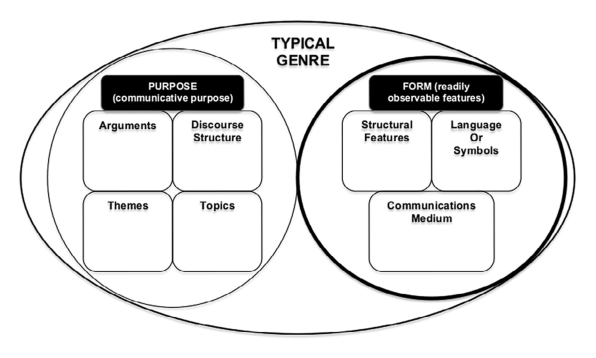
\includegraphics[scale=0.95]{Figures/Sotlen_diagram.eps}
		\caption{Stolen Imag.}
		\label{fiig:Stolen}
	\end{center}
\end{figure}







A very recent research on Cross-Lingual Genre Classification showed that it is possible to get very good results when an ML model is trained with a corpus samples of one language and then testing the trained model to an other. However, the evaluation framework was closed-set and the relation of the languages seems to be of a great importance for the accuracy performance of the model. That is, in some cases it was important the language to be of the same group for example the Roman or the Slavic group of languages and for others was not. Some times oddly the performance was dropping when the language was form the same language group \parencite{nguyen2019cross}.

Web Genre Identification (WGI) concerns the association of web pages with labels that correspond to their form, communicative purpose and style rather than their content. The ability to automatically recognize the genre of web documents can enhance modern information retrieval systems by enabling genre-based grouping/filtering of search results or building intuitive hierarchies of web page collections combining topic and genre information \parencite{Braslavski2007,Rosso2008,de2009genre}. For example, a search engine can provide its users with the option to define complex queries (e.g., blogs about machine learning or eshops about sports equipment) as well as the option to navigate through results based on genre labels (e.g. social media pages, web shops, discussion forum, blogs, etc). The recognition of web genre can also enhance the effectiveness of processing the content of web pages in information extraction applications. For example, given that a set of web pages has to be part-of-speech tagged, appropriate models can be applied to each web page according to their genre \parencite{Nooralahzadeh2014}. However, research in WGI is relatively limited due to fundamental difficulties emanating from the genre notion itself.


The most significant difficulties in the WGI domain are: (1) There is not a consensus on the exact definition of genre \parencite{crowston2011problems}; (2) There is not a common genre  palette that comprises all available genres and sub-genres \parencite{santini2011cross,mehler2010genres_on_web,mason2009n,sharoff2010web}, moreover, genres are evolving in time since new  genres are born or existing genres are modified \parencite{Boese2005}; (3) It is not clear whether a whole web page should belong to a genre or sections of the same web page can belong to  different genres \parencite{jebari2015combination,madjarov2015web}; (4) Style of documents is affected by both genre-related choices and author-related choices \parencite{petrenz2011stable,Sharroff2010}. As a result, it is hard to accurately distinguish between personal style characteristics and genre properties when style is quantified.

Genre means "genus" in the Greek language and for the text focused studies (either traditional linguistics or computational) mainly means style. The main utility of the genre taxonomy is for speeding up the communication in a broader sense. 

Starting with two cases outside the computer science the genre taxonomy is very useful in English 

One (REF) from the discipline of the \textit{English for Academic Purposes} (EAP) where it was vividly discussed the divergence in the genre taxonomies between the difference academic disciplines and reasoned the utility of the genre taxonomy for enabling the teachers and the students to improve their rhetorical and written language with the purpose of improving the teaching procedure. What is important to note for this study is the conclusion that the same genre-type can be very different for the communication purpose, i.e. as text identity carrier, but it can also contain the same style and other language properties when the purpose is similar, for example the article of new paper and an article form a magazine where one can claim that they are a different genre-type although they governed by the same linguistic properties.

The types of their study genre taxonomy mainly focused on the \textit{purpose} of the students written context and less on the \textit{style}, thus their genre-types where \textit{Creative Writing, Response Paper, Critique/Evaluation, Argumentative Essay, Report, Research Paper and Proposal}. Their study was a manual statistical process, similar to a \textit{Data Mining} process where grammatical features were counted in the texts. Then these features where indicating the score for each of the four (4) dimensions which has been qualitatively predefined. The counting process was using a heuristic computational tagger, named as Biber tagger (see Biber 1988 or ??? *** Genre variations in student .... (paper)).   
  
  ***
Genres, in textual sense, is sometimes defined as group of texts of documents that share a communicative purpose, as determined by the \textit{discourse community} which produces and/or reads them. "In \textbf{structural}terms, genre are social institutions that are produced, reproduced, reproduced or modified when \textit{human agents} draw on genre rules to engage in organizational communication".

"Layout in organizational communities cause people to focus perceptually on key parts of the text and our \textbf{empirical research has previously demonstrated that people use layouts and other related cues to focus on key parts of the text.}"
***


On the other hand and other research lying in the discipline of cognitive computing an health research they found humans are recognizing the genre type of a document or web-page using other cognitive processes relates mostly to the formatting of the text. Particularly they used as well configured apparatus for tracking the eyes movement while the recognition effort, where they fount that the eyes where following specific paths and where stopping to special landmarks on the text. They have concluded that the process of genre recognition was mostly related to the format and not the context, in addition they statistically measured that they previews experience was not related to the recognition process. Although it was the previews knowledge of the text formatting was accelerating the process. However, on the opinion of the authors of this study the genre recognition is a more deep process, thus as one can concluded by reading their study the landmarks they are referring into seems to be the only context combined with the formatting of the text that the human brain is requiring for identifying the genre-type. Given that their study is focused on the e-mail genres where formatting options compare to the web or textbooks is rather limited is advocating the conclusion that the minimum context is required for identifying the genre-type.

They are discussing of tree main perception (psychology) theories, i.e. Gestaltism (or Gestalt psychology), Ecological and Constructivism, which are the theories which can interpret the perception procedures, it this case the eye movement on the texts, to the cognition process for identifying the genre types of the texts. The perception procedure includes some eye movements mainly doing two tasks, \textit{scanning} and \textit{skimming}. Theses two procedures are irrespective of the belief of the supported interpretation theory related to the internal thought process for making a genre taxonomy decision. Scanning is the process where more or less we are trying to locate information of interest where the information has a homogeneous property, such as the a phone number in phone-book list. Skimming is the process where we are trying to locate information of interest where the information is raw or without a specific form, such as names, verbs, or phrases that is related to the abstract related concept in order to decide whether the text is matches and worth farther reading. 

The process of scanning and especially skimming in practice follows some specific eye movements, i.e. Fixation and Saccadic. Saccadic is the process while scanning or skimming that the eye is jumping around to the text, while Fixation is the process where the eye remains focused for a while. One can resemble the process like navigation where the eye is constantly moving while is focused for small fragments of time in landmarks of interest.
  
As \textit{Web Search} from an extension of IR because the main subject under investigation \parencite{manning2008introduction}, \textit{Web page Genre Classification } is becoming the main subject of document classification research.

Blogs is a genre-type has attracted as special interest on its own, in differed domains such as in sociology, psychology, linguistics and mostly in computational linguistics and WGI. There are several blogs' properties of interest of the research and  also blogs having their own sub-genre taxonomy. Blog-taxonomy general genres are \textit{Filter, Personal-diary} and \textit{Notebook} and other related to the authors group of styles such as \textit{Reflective, Narrative, Emotional, ratioal} and \textit{Personal , Non-Personal}. The thought research on the blog-types classification has delivered a set of special linguistic and web-page structural properties which are increasing the performance of the closed set classification. Details for this linguistic properties used for specially for blogs sub-taxonomy classification are described in section \ref{chap:relevant_work:sec:features:subsec:heuristics} \parencite{virik2017blog,hoffmann2012cohesive,hoffmann2012cohesive,derczynski2014social,qu2006automated}. 

Most previous work in WGI follows a typical closed-set text categorization approach where, first, features are extracted from documents and, then, a classifier is built to distinguish between classes. Attention is paid to the appropriate definition of features that are able to capture genre characteristics and should not be affected by topic shifts or personal style choices. 

